\documentclass[11pt,a4paper]{article}
\usepackage[T1]{fontenc}
\usepackage[utf8]{inputenc}
\usepackage{lmodern,microtype}
\usepackage[a4paper,margin=24mm,headheight=15pt]{geometry}
\usepackage{amsmath,amssymb,amsthm,mathtools}
\usepackage{booktabs,longtable,array,tabularx,multirow}
\usepackage{graphicx,xcolor,enumitem,fancyhdr,float}
\usepackage[hyphens]{url}
\definecolor{ink}{HTML}{17384C}
\definecolor{muted}{HTML}{516877}
\definecolor{pale}{HTML}{EEF4F7}
\usepackage[colorlinks=true,linkcolor=ink,citecolor=ink,urlcolor=ink]{hyperref}
\hypersetup{pdftitle={Dual Certificates and Forced Quadrilateral Propagation for Unknot Recognition},pdfauthor={ProveIt research continuation prepared with ChatGPT},pdfsubject={Exact normal-surface certificates, parameterized algorithms, and conditional quasi-polynomial complexity}}
\usepackage{listings}
\lstset{basicstyle=\ttfamily\small,breaklines=true,columns=fullflexible,keepspaces=true,frame=single,framerule=.25pt,rulecolor=\color{muted},backgroundcolor=\color{pale},showstringspaces=false}
\setlength{\parskip}{4pt}
\setlength{\parindent}{0pt}
\setlength{\emergencystretch}{2em}
\setlist{itemsep=2pt,topsep=4pt,leftmargin=*}
\renewcommand{\arraystretch}{1.15}
\newtheorem{theorem}{Theorem}[section]
\newtheorem{lemma}[theorem]{Lemma}
\newtheorem{proposition}[theorem]{Proposition}
\newtheorem{corollary}[theorem]{Corollary}
\theoremstyle{definition}
\newtheorem{definition}[theorem]{Definition}
\newtheorem{example}[theorem]{Example}
\theoremstyle{remark}
\newtheorem{remark}[theorem]{Remark}
\newcommand{\R}{\mathbb R}
\newcommand{\Q}{\mathbb Q}
\newcommand{\Z}{\mathbb Z}
\newcommand{\F}{F}
\newcommand{\Ftwo}{\mathbb F_2}
\newcommand{\poly}{\operatorname{poly}}
\newcommand{\supp}{\operatorname{supp}}
\newcommand{\rank}{\operatorname{rank}}
\newcommand{\cone}{\operatorname{cone}}
\newcommand{\ch}{\chi}
\newcommand{\status}[1]{\texttt{#1}}
\newcommand{\code}[1]{\texttt{\detokenize{#1}}}
\newcommand{\baseline}{\texttt{3a90fb34146c915328ab8eac6250cc2514f74ed0}}
\pagestyle{fancy}
\fancyhf{}
\fancyhead[L]{\small\color{muted}ProveIt / Unknot recognition}
\fancyhead[R]{\small\color{muted}Dual certificates and propagation}
\fancyfoot[C]{\small\thepage}
\renewcommand{\headrulewidth}{.3pt}
\begin{document}
\hypersetup{pageanchor=false}
\begin{titlepage}
\vspace*{12mm}
{\large\color{muted}TOPOLOGY / ALGORITHMIC RESEARCH\par}
\vspace{7mm}
{\huge\bfseries\color{ink}Dual Certificates and Forced Quadrilateral Propagation for Unknot Recognition\par}
\vspace{6mm}
{\Large A support-aware LP continuation, a proved dense-family separation, and conditional quasi-polynomial search\par}
\vspace{9mm}
{\large Research continuation for Vladimir Reshetnikov's ProveIt project\par}
{\normalsize Prepared with ChatGPT \quad | \quad 9 October 2026\par}
\vspace{10mm}
\begin{abstract}
\noindent
The previous quadrilateral-support kernel gives small exact normal-surface systems, but complete ray enumeration and exponential type selection remain different bottlenecks. This continuation develops three certificate-producing improvements and makes the remaining asymptotic obligation explicit. First, canonical positive-Euler existence in a compatible sector is decided by a family of rational linear programs, with at most $4k+1$ anchor objectives when the triangulation has one global vertex and the sector allows $k$ quadrilateral coordinates. Exact Farkas multipliers certify an entire negative sector without enumerating its rays; a componentwise envelope and certified dual reuse can reduce the work further. Second, primitivity and one modular rank witness certify connectedness of a standard extreme ray, allowing essential discs to be verified without a general component census. Third, mandatory-type implications give a monotone propagation closure and a strong backdoor parameter for the remaining quadrilateral choices.

We prove that the Fibonacci layered solid tori have propagation backdoor zero for every number of tetrahedra, despite their linear essential-disc support obstruction and exponentially large coordinates. A supplied backdoor of size $b$ yields $A(T)3^b\poly(t)$ exact positive-Euler search with a polynomial rational-LP oracle; finding an unknown backdoor costs $A(T)(3t)^{O(b)}\poly(t)$, where $A(T)=4t$ for one vertex. This gives a precise conditional route to quasi-polynomial unknot recognition through the classical search-and-crush framework. An unused-tetrahedron obstruction limits the strong parameter; a policy-dependent deciding-set refinement permits early positive termination. No logarithmic bound for arbitrary knot exteriors is proved.

The accompanying additive Python prototype has independent arithmetic checkers, explicit inconclusive outcomes under caps, frozen independent normal-surface oracles, adversarial examples, and reproducible measurements. The shipped simplex engine is exact but has no proved polynomial pivot bound. The report separates local theorems, executable evidence, classical ingredients, and the unresolved global theorem throughout.
\end{abstract}
\vfill
{\small\color{muted}Repository snapshot: \baseline\par}
{\small\color{muted}Primary paths: \code{Topology/UnknotRecognition} and \code{docs/incoming}.\par}
\end{titlepage}
\clearpage
\pagenumbering{roman}
\hypersetup{pageanchor=true}
\tableofcontents
\clearpage
\pagenumbering{arabic}
\section{The result and its scope}\label{sec:overview}

The most useful next performance step is to stop treating enumeration of every normal ray as the default way to answer a positive-Euler existence query. An exact linear program can either supply one useful ray or certify a whole cone negatively. The unresolved exponential work then has a more specific location: selecting compatible quadrilateral types after all sound implications have been exhausted. This report develops that separation mathematically and implements it in the ProveIt normal-surface research code.

The resulting contribution is a combination of local algorithms, a structural parameter, an infinite-family theorem, and an executable audit. It is not a proof of general quasi-polynomial running time. That distinction determines both the statements below and the meanings of the code's return values.

\subsection{What this continuation establishes}

\begin{enumerate}
\item \textbf{A sector decision method independent of matching nullity.} For a supplied compatible sector with $k$ quadrilateral coordinates, the canonical Euler functional is the maximum of $P$ linear objectives. The contracted anchor count satisfies
\[
 P\le (1+4k/\nu)^\nu\quad(\nu>0),\qquad
 P\le 2^{4k},
\]
where $\nu$ is the number of active global vertices; $P=1$ if $\nu=0$. For one global vertex, $P\le4k+1$. Positive-Euler existence can therefore be decided by polynomially many rational LPs in a one-vertex sector, with no assumption that its matching nullity is small.
\item \textbf{Short negative proofs.} Each unsuccessful objective admits a homogeneous Farkas multiplier. Complete anchor coverage turns these local inequalities into a source-bound negative sector certificate. A single upper-envelope multiplier sometimes replaces the whole list. Neither verification route invokes ray enumeration.
\item \textbf{A restricted, cheaper disc proof.} Given a primitive integer standard normal ray, exact matching plus rank $s-1$ on its $s$ positive columns proves that the represented surface is connected. Euler characteristic one, nonempty boundary and nonzero boundary class modulo two then certify an essential disc in the supplied torus-boundary manifold. A modular rank witness avoids a general component census on this class of inputs.
\item \textbf{A propagation parameter with a proved non-sparse family.} Mandatory quadrilateral types can be justified by negative LP certificates for coordinate faces. These implications preserve every admissible positive-Euler solution and have a confluent exhaustive closure. The Fibonacci layered solid tori have strong propagation backdoor zero for all $t$, although their essential vertex discs cannot have sublinear quadrilateral support. Conversely, any canonical positive surface avoiding $t-k$ tetrahedra forces the strong parameter to be at least $t-k$. A deciding-set refinement retains early positive termination and has the same parameterized search bounds for a fixed polynomial LP policy.
\item \textbf{An explicit conditional asymptotic theorem.} A logarithmic strong backdoor bound, maintained through a complete topological continuation and used with polynomial-time exact LP, would give quasi-polynomial recognition. The package does not establish that structural bound or implement the complete certified crushing continuation.
\end{enumerate}

\subsection{Which earlier results are being continued}

The main dependency is the incoming report \emph{Quadrilateral Support Kernels and Certified Normal-Disc Discovery} and its archive \code{unknot_quadrilateral_support_kernel_20261009.zip} \cite{priorKernel}. Its contraction, canonical lifting, mixed-minor height estimate, low-nullity ray methods and dense layered-torus obstruction are treated as earlier work. The two modules \code{normal_sector.py} and \code{normal_sector_verify.py} are included unchanged as explicit dependencies. They are not part of the maintained runtime at the pinned commit.

The other incoming continuations matter because they distinguish the cost of choosing a surface from the cost of processing one already supplied: compiled certificates, orbit transfer, sparse incidence, persistent elimination and topology spectra attack different portions of that pipeline. The present changes do not replace their general component or boundary machinery. They add a short ray-specific proof route and a decision query that avoids unnecessary ray output. The package's source inventory records the ten relevant incoming archives inspected, so the continuation is anchored to the actual intake state rather than to report titles alone.

The maintained source snapshot is \baseline. Its existing normal-surface validation and component APIs provide the geometric trust boundary and the comparison implementation. All new files are delivered additively, with a patch for later review. No conclusion in this report depends on applying an incoming patch silently to the maintained tree.

\subsection{Relation to the published algorithmic framework}

Linear programming, zero-triangle anchors, support descent and greedy LP branching are classical ingredients here. Burton--\"Ozlen explicitly use them in their branching recognizer; their Algorithm~9, Lemmas~7--10 and Theorems~11--12 in arXiv version~3 are the relevant references \cite{BO}. The present claims concern the contracted anchor count, dual certificate interfaces and bounds, the precise propagation parameter, its all-$t$ Fibonacci separation, and this implementation. They do not claim that LP normal-surface search or forced branching is newly invented.

Canonical lifting in quadrilateral coordinates belongs to the established Q-theory literature \cite{Tollefson,BurtonQ}. Essential-disc vertex results are also classical \cite{HLP,Suh}. We give the needed elementary extremality and connectedness arguments explicitly because they delimit the new short checker.

Current quasi-polynomial announcements also require care. Lackenby's detailed Oxford talk displays $2^{O((\log n)^3)}$, equivalently $n^{O((\log n)^2)}$ \cite{LackenbyTalk}. The July 2026 hierarchy paper expressly leaves some algorithms insufficiently specified for a running-time estimate in Section~9 \cite{Lackenby2026}. These sources motivate a serious quasi-polynomial programme; they do not supply a complexity theorem for this Python prototype. In this report ``quasi-polynomial'' means $\exp((\log n)^{O(1)})$, with the exponent stated whenever a sharper conditional bound is available.

\subsection{A claim ledger}

\begin{center}\small
\begin{tabularx}{\textwidth}{@{}>{\raggedright\arraybackslash}p{.23\textwidth}>{\raggedright\arraybackslash}X>{\raggedright\arraybackslash}p{.24\textwidth}@{}}
\toprule
Claim & Evidence & Status\\
\midrule
Fixed-sector positive-Euler decision & Anchor/max theorem and Farkas alternative & Proved; polynomial for bounded vertex count with polynomial LP\\
Primitive-ray disc verification & Exact geometry, gcd, modular rank and boundary homology & Proved on the stated domain; implemented\\
Mandatory-type closure & Preservation and monotone fixed-point proof & Proved; bounded prototype implemented\\
Fibonacci backdoor zero & Symbolic matching and Euler identities for arbitrary $t$ & Proved infinite family\\
Small general backdoor & No universal estimate obtained & Open research question\\
Quasi-polynomial complete recognizer & Conditional backdoor theorem plus complete topological continuation & Conditional; not delivered as a finished recognizer\\
Polynomial implementation runtime & Exact Bland simplex, measured caps and operation counts & Not proved; polynomial-oracle theorem kept separate\\
\bottomrule
\end{tabularx}
\end{center}

\section{Exact setting, encoding and the inherited kernel}\label{sec:setting}

\subsection{Input and topological trust boundary}

Let $T$ be a finite generalized triangulation with $t$ tetrahedra. Faces may be identified within a tetrahedron, and distinct local edges or corners may represent the same global cell. The implemented validators require a connected compact orientable three-manifold with exactly one boundary component, a torus. They check the face pairing data, edge links, vertex links, orientability and boundary topology. Interior vertex links are spheres and boundary vertex links are discs. Ideal triangulations with unfilled cusps are outside this API's domain.

The input encoding lists face pairings and permutations, so its combinatorial length is $O(t\log t)$. Normal coordinates and rational certificates are encoded in binary; an operation on an integer with exponentially large value is not a unit-cost operation. We write $L$ for a bound on coordinate bit length when analysing a supplied surface. The ray certificate uses a source-coordinate fingerprint including exact values. Sector and propagation certificates hash the source triangulation and replay their explicit coordinates or duals. These digests bind a proof to its input. Correctness comes from replaying the mathematical conditions, not from treating a digest as a topological proof.

A validated torus-boundary triangulation is not automatically known to be a knot exterior in $S^3$. The statement ``this surface contains an essential disc'' concerns the supplied manifold. To infer unknottedness of a particular diagram requires a separate checked correspondence from that diagram to this exterior. The maintained project contains exterior and transformation interfaces, but the new modules intentionally expose surface-level predicates. A negative result for one sector cannot be promoted to a statement about all surfaces, and a positive Euler value cannot be promoted to a disc verdict.

\subsection{Standard coordinates and canonical surfaces}

Write a standard normal vector as
\[
 x=(a_{iv},q_{ij})\in\R_{\ge0}^{7t},\qquad
 0\le i<t,\quad 0\le v<4,\quad 0\le j<3.
\]
There are four triangle types and three quadrilateral types in each tetrahedron. Let $M_0x=0$ be the integer matching equations. For each paired face and each of its three corners, the number of arcs cutting off that corner must agree on both sides. These equations remain meaningful even if several quadrilateral types are temporarily allowed in one tetrahedron. Such a point is a relaxation point, not yet an embedded normal surface. Admissibility additionally requires at most one positive quadrilateral type in each tetrahedron.

An integral admissible matching vector represents a normal surface. Its Euler characteristic is a linear function on the matching space. We use a particularly transparent integer extension: count one normal vertex at one chosen local representative of each global ambient edge, one normal edge at one representative of each global ambient face, and one normal face for each normal disc. Matching makes these counts independent of the chosen representative on the solution space. Before contraction, triangle coefficients lie in $[-2,4]$ and quadrilateral coefficients in $[-3,5]$. Each coefficient consists of one disc contribution, at most three or four subtracted face contributions, and at most three or four selected edge contributions.

For a global vertex $v$, let $L_v$ denote its vertex-link vector. Subtracting the minimum triangle coordinate around $v$ removes a maximal nonnegative multiple of $L_v$. This operation at all vertices gives the \emph{canonical} representative of a fixed quadrilateral vector. Equivalently, a nonnegative matching vector is canonical exactly when at least one triangle coordinate at every global vertex is zero. Here canonicality means removal of vertex-link components; it does not mean a canonical triangulation or a canonical knot diagram.

\subsection{A supplied compatible sector}

A compatible sector is a list
\[
 S\subseteq\{(i,j):0\le i<t,\ 0\le j<3\}
\]
containing at most one pair for each $i$. Put $k=|S|$. Every quadrilateral coordinate outside $S$ is fixed to zero; a type listed in $S$ is \emph{allowed}, not required to be positive. In particular, the zero-quadrilateral face is included in every full singleton-type assignment. This convention is what makes three branches per tetrahedron sufficient.

The incoming support-kernel construction \cite{priorKernel} treats each matching equation as a difference between two triangle coordinates plus an integer linear form in the allowed quadrilaterals. Equations with zero quadrilateral label identify their triangle endpoints. Contracting those equalities and discarding isolated vertex-link factors produces a matrix
\begin{equation}\label{eq:small-kernel}
 C_S=\{z\ge0:Mz=0\},\qquad
 M\in\Z^{m\times N},\qquad m\le4k,\quad N\le9k.
\end{equation}
Each retained row has a nonzero quadrilateral label. A quadrilateral meets four faces, so the total number of its nonzero arc incidences is at most four; summing gives $m\le4k$. Nonzero-labelled loops remain as consistency rows. Identifications and coefficient cancellations cannot increase the incidence bound. The triangle block is a graph incidence matrix with rows and columns transposed, hence is totally unimodular. Each quadrilateral column has $\ell_1$ norm at most four.

The retained triangle classes are grouped by global vertex. Let $G_v$ have size $p_v\ge2$, and let $\nu$ be the number of these active groups. An inactive singleton group is an independent link direction; its value is zero in a canonical representative. These removed factors are not silently counted as possible positive-Euler witnesses.

\begin{lemma}[Sharper count of anchor classes]\label{lem:anchor-count}
The active groups satisfy
\[
 \sum_v(p_v-1)\le4k.
\]
Consequently, with the empty product interpreted as one,
\begin{equation}\label{eq:anchor-count}
 P:=\prod_v p_v\le
 \begin{cases}(1+4k/\nu)^\nu,&\nu>0,\\1,&\nu=0,
 \end{cases}
 \qquad P\le2^{4k}.
\end{equation}
For a one-global-vertex triangulation, $P\le4k+1$.
\end{lemma}
\begin{proof}
The original triangle graph at a global vertex is connected: it is the face-adjacency graph of its connected vertex link. Contraction preserves connectivity. A connected graph on $p_v$ retained classes has at least $p_v-1$ edges; loops do not help connect distinct classes. These edges are among the at most $4k$ retained matching rows. Sum over vertices. The arithmetic--geometric mean inequality applied to the $p_v$ proves the first estimate. The elementary inequality $p\le2^{p-1}$ for integers $p\ge2$ proves the second. With at most one active group, its size is at most $4k+1$.
\end{proof}

\subsection{Potentials and the full quadrilateral consistency matrix}

Choose a spanning tree in each retained triangle graph. Integrating the quadrilateral labels along the tree expresses a triangle class $c$ at vertex $v$ as
\[
 a_c=\alpha_v+\ell_c(q),
\]
where $q\in\R^k$ is the allowed quadrilateral vector and $\ell_c$ is an integer linear form. The remaining matching equations give the cycle-consistency system $Rq=0$. Define
\begin{equation}\label{eq:Q}
 Q_S=\{q\in\R^k:q\ge0,\ Rq=0\}.
\end{equation}
This $R$ includes the entire finite triangle-graph consistency condition. It must not be replaced without proof by a different ideal or spun-normal Q-matching system.

The canonical lift is
\begin{equation}\label{eq:canonical-lift}
 \F(q)_c=\ell_c(q)-\min_{d\in G_v}\ell_d(q),\qquad
 \F(q)_{ij}=q_{ij}.
\end{equation}
Coordinates at removed singleton groups are zero. Integer $q$ has integer potentials and therefore an integer lift. All freedom in a nonnegative lift of $q$ is addition of nonnegative vertex links. This is the finite canonical-extension picture from Q-theory, specialized to the exact contracted coordinates \cite{Tollefson,BurtonQ}.

\begin{lemma}[Primitivity and extremality under lifting]\label{lem:lift-extreme}
For nonzero integral $q\in Q_S$, $\gcd(\F(q))=\gcd(q)$. If $q$ spans an extreme ray of $Q_S$, then $\F(q)$ spans an extreme ray of the standard normal cone with all off-sector quadrilaterals zero, and hence of the full nonnegative standard matching cone.
\end{lemma}
\begin{proof}
The quadrilaterals are a subvector of the lift, so the gcd of the lift divides the gcd of $q$. Conversely, any common divisor of $q$ divides all integral potentials and their minima, and therefore all lifted triangle entries. For extremality, suppose $\F(q)=u+w$ with $u,w$ nonnegative matching vectors. Their quadrilateral projections are nonnegative vectors in $Q_S$ adding to $q$; extremality gives $\pi(u)=\alpha q$ and $\pi(w)=(1-\alpha)q$ for $0\le\alpha\le1$. Positive homogeneity gives $\F(\alpha q)=\alpha\F(q)$. The remaining parts of $u$ and $w$ are nonnegative vertex-link combinations. A zero canonical triangle at each vertex forces all these link coefficients to vanish. Thus $u,w$ lie on the same ray. Finally, setting coordinates to zero is passage to a face of a nonnegative cone, and an extreme ray of a face is an extreme ray of the original cone.
\end{proof}

The matching nullity $d=\dim\ker R$ remains useful for choosing an enumeration algorithm when all rays are actually needed. The new existence test below makes no small-$d$ assumption. Removing that assumption from a query is different from bounding the number of rays or the number of compatible sectors.

\section{Positive-Euler search by anchor LPs and dual certificates}\label{sec:sector-lp}

\subsection{A union of anchored coordinate faces}

Let $M$ be the contracted standard matrix in \eqref{eq:small-kernel}, and let $c$ be the integer Euler covector obtained by expanding a contracted vector back to standard coordinates. For each tuple $a=(a_v)_v\in\prod_vG_v$, set its chosen triangle entries to zero. Let $J_a$ be the surviving columns and define
\begin{equation}\label{eq:anchor-lp}
 \mathcal L_a=\{z\in\R^{J_a}:z\ge0,\ M_{J_a}z=0,\ c_{J_a}^{T}z\ge1\}.
\end{equation}

\begin{theorem}[Support-sensitive anchored decision]\label{thm:anchor}
A compatible sector contains a canonical normal surface of positive Euler characteristic if and only if $\mathcal L_a$ is nonempty for some anchor tuple $a$. Consequently this query is decidable by $P$ rational LP feasibility tests with $O(k)$ variables and rows, after polynomial preprocessing in $t$. For one global vertex the query has polynomial bit complexity when implemented with a polynomial-time rational-LP algorithm.
\end{theorem}
\begin{proof}
Canonicality is precisely the existence of a zero triangle coordinate in each global vertex group. Equality contraction preserves these zero conditions. Thus the canonical nonnegative matching vectors form the union of the anchored coordinate faces. Positive Euler is homogeneous: any positive real value can be scaled to at least one. Conversely, a feasible rational point in \eqref{eq:anchor-lp} can be multiplied by a common denominator to produce integral matching coordinates. Compatibility is already enforced by the sector. Rational feasibility suffices because the polyhedron has rational defining data. The number of tuples is given by Lemma~\ref{lem:anchor-count}. The matrix and objective have polynomial encoding length; the result follows from rational LP complexity \cite{Khachiyan}.
\end{proof}

The theorem decides \emph{whether at least one} canonical positive-Euler surface exists. It does not list every such ray. Enumeration can still be required by a downstream task that needs alternatives, all boundary slopes, or a complete output set. It is inappropriate to claim a speedup for such a task merely because this weaker query became cheaper.

\subsection{A complete negative result is a list of inequalities}

\begin{theorem}[Homogeneous dual alternative]\label{thm:dual}
For an anchor tuple $a$, the system $\mathcal L_a$ is empty if and only if there is a rational vector $y_a$ such that
\begin{equation}\label{eq:standard-dual}
 M_{J_a}^{T}y_a\ge c_{J_a}
\end{equation}
componentwise. A multiplier for every anchor tuple is a complete negative certificate for the sector.
\end{theorem}
\begin{proof}
If \eqref{eq:standard-dual} holds, then every nonnegative kernel vector satisfies
\[
 c_{J_a}^{T}z\le y_a^{T}M_{J_a}z=0,
\]
contradicting the last inequality in \eqref{eq:anchor-lp}. For the converse, the polar of the polyhedral cone $\{z\ge0:M_{J_a}z=0\}$ is the sum of the row space of $M_{J_a}$ and the nonpositive orthant. If the objective is nonpositive on that cone, it therefore has the form $M_{J_a}^{T}y_a-s$, $s\ge0$. All defining data are rational, so a rational multiplier exists. This is the homogeneous Farkas alternative. The anchor theorem supplies complete coverage.
\end{proof}

The verifier reconstructs the anchor product itself. An asserted count, a sample of anchors, or a list of successfully tested anchors is insufficient. In the implementation, ordinary negative certificates list the deterministic Cartesian product in order; missing, repeated, reordered or foreign tuples are rejected. The checker rebuilds matching rows and Euler coefficients from the source and checks exact rational inequalities. The shipped checker uses the equivalent cycle-coordinate multipliers introduced below. It never asks the producer whether a branch was exhausted.

\begin{proposition}[A sharp numeric bound in anchored standard coordinates]\label{prop:dual-bits}
For each negative anchor query, a multiplier can be chosen with at most $4k$ nonzero entries, denominators at most $4^k$, and numerator absolute values at most $64kt4^k$. A full anchored-standard negative proof therefore needs
\begin{equation}\label{eq:dual-bits}
 O\bigl(Pk(k+\log t+\log(k+1))\bigr)
\end{equation}
numeric bits, apart from source and indexing metadata.
\end{proposition}
\begin{proof}
Every square minor of the contracted matrix containing $a$ quadrilateral columns has absolute determinant at most $4^a$. Expand in those columns: their $\ell_1$ norms are at most four, and the remaining triangle minor is zero or has absolute determinant one because the triangle block is totally unimodular. This recovers the mixed-minor estimate used in the preceding report \cite{priorKernel}.

Let $r=\rank M_{J_a}\le4k$ and retain $r$ independent rows, denoted $A$. Their row space is unchanged. The nonempty polyhedron $\{u:A^Tu\ge c_{J_a}\}$ is pointed, since $A^T$ has trivial kernel. A nonempty pointed polyhedron has a vertex. At a vertex, choose $r$ linearly independent active column inequalities. The resulting square matrix has nonzero integer determinant of absolute value at most $4^k$. A Cramer numerator expands along the inserted objective row into at most $r$ terms. The remaining minors have absolute value at most $4^k$, and $\|c\|_\infty\le16t$: at most $4t$ triangle coefficients of magnitude at most four are identified. Hence the numerator bound is $r(16t)4^k\le64kt4^k$. Put zeros on the omitted original rows. Reducing fractions can only decrease numerator and denominator magnitudes. Rank zero uses the empty multiplier and direct comparison $c_{J_a}\le0$. Taking binary lengths gives \eqref{eq:dual-bits}.
\end{proof}

This bound proves that the negative proof need not encode an enormous enumeration history. It is an existence bound for a suitable anchored-standard dual. The prototype below solves the smaller cycle-coordinate LPs, whose stored duals satisfy a generic polynomial bit bound. We do not assert that the actual cycle-coordinate multipliers satisfy the sharper $4^k$ bound without a proved change-of-basis estimate.

\subsection{The equivalent quadrilateral formulation}

The potential description makes all anchor objectives share the same feasible cone. Let $\lambda(q)$ be the Euler value of the lift using zero reference offsets, before subtracting vertex minima. Write $w_v=\chi(L_v)$, so $w_v=1$ for boundary vertices and $w_v=2$ for interior vertices. The canonical Euler functional is
\begin{equation}\label{eq:canonical-euler}
 g(q):=\chi(\F(q))=\lambda(q)-\sum_v w_v\min_{c\in G_v}\ell_c(q).
\end{equation}
It is generally piecewise linear, not one globally linear functional of $q$.

\begin{theorem}[Maximum-of-objectives formulation]\label{thm:max-objectives}
Define
\[
 h_a(q)=\lambda(q)-\sum_v w_v\ell_{a_v}(q).
\]
Then $g(q)=\max_a h_a(q)$ on $Q_S$. Therefore $g$ is positive somewhere on $Q_S$ if and only if at least one objective $h_a$ is positive on
\begin{equation}\label{eq:normalized-Q}
 \{q\ge0:Rq=0,\ \mathbf1^Tq\le1\}.
\end{equation}
A complete negative certificate consists of multipliers satisfying $R^Ty_a\ge h_a$ for all $a$.
\end{theorem}
\begin{proof}
Each $w_v$ is positive, so replacing the minimum in \eqref{eq:canonical-euler} by any particular potential can only decrease the value. Choosing a minimizing potential independently in every group attains equality. Nonzero positive values can be scaled into \eqref{eq:normalized-Q}; the zero vector has value zero. Apply the homogeneous dual alternative to $R$ and $h_a$.
\end{proof}

No extra inequalities asserting that the chosen anchors are actual minima are needed. If an anchor objective is positive at $q$, the canonical objective is at least as large; if the canonical objective is positive, actual minima supply a successful tuple. This observation removes a potentially expensive and unnecessary cell arrangement from the decision problem.

The sign of each vertex-link Euler characteristic matters for this maximum identity. A zero link weight disappears, while a negative weight changes the relevant minimum into a concave contribution. The direct anchored-standard theorem uses zero-coordinate faces and does not depend on that sign argument. The present implementation only accepts the finite sphere/disc-link setting, so there is no hidden extension to arbitrary ideal triangulations.

\subsection{Obtaining a ray, rather than an arbitrary feasible point}

The normalized polytope \eqref{eq:normalized-Q} is compact. Every nonzero vertex of it lies on $\mathbf1^Tq=1$ and spans an extreme ray of $Q_S$. A positive basic feasible point therefore gives a Q-ray, even if it does not maximize the objective. Clearing denominators and dividing by the gcd produces its primitive integral generator. Lemma~\ref{lem:lift-extreme} then gives a primitive standard ray after canonical lifting.

The shipped simplex implementation begins with a feasible all-slack basis for $Rq\le0$, $-Rq\le0$ and $\mathbf1^Tq\le1$. It uses exact fractions and Bland's finite pivot rule \cite{Bland}, and stops as soon as its basic objective value becomes positive. For a nonpositive optimum it extracts a homogeneous dual and checks the dual inequalities before returning. Feasibility, primitivity and exact Euler characteristic are also checked before a positive result is exposed.

A general polynomial LP routine might return an interior feasible point. To recover an extreme positive ray without assuming its output is basic, first work in the anchored standard formulation \eqref{eq:anchor-lp}. Preserve all current zero coordinates and repeatedly test whether one further positive coordinate can be set to zero while retaining the linear constraint $c^Tz\ge1$. Keep every successful deletion. At most $N$ tests yield minimal positive support. If that support face had dimension greater than one, its extreme-ray decomposition would contain a positive-Euler ray on smaller support, a contradiction. This support-descent mechanism is classical \cite{BO}. It makes the theoretical polynomial-oracle statement independent of a particular LP solver's output convention.

\subsection{An inexpensive envelope and safe reuse of duals}

Let $h_a$ also denote the coefficient vector of the corresponding linear form. Set
\begin{equation}\label{eq:envelope}
 u_j=\max_a(h_a)_j
     =\lambda_j-\sum_vw_v\min_{c\in G_v}(\ell_c)_j.
\end{equation}
Because $q\ge0$, every $h_a(q)\le u^Tq$, so $g(q)\le u^Tq$. One multiplier $R^Ty\ge u$ proves that the entire sector has no canonical positive-Euler surface. The coefficientwise maximum can be constructed without enumerating the anchor product.

This envelope is sufficient for a negative conclusion; positivity of the envelope proves nothing by itself. For example, let
\[
 R=(1,-1),\qquad h_1=(1,-2),\qquad h_2=(-2,1).
\]
The nonnegative kernel consists of $(s,s)$, $s\ge0$. Both anchor objectives equal $-s$, so $g=-s$, but $u=(1,1)$ gives $u^Tq=2s$. The prototype tests this failure mode and falls back to the actual anchor objectives after a positive envelope LP. It cannot return a surface merely from the positive upper bound.

Duals can also be reused safely. If a previous multiplier has $b=R^Ty$, then it certifies every later objective $h$ with $h\le b$ componentwise. This requires only a coordinate comparison. The implementation initially caches the zero dual, which immediately handles objectives with nonpositive coefficients. Reusing a dual does not remove the anchor from an ordinary negative certificate: the checker still verifies full coverage. Duplicate multipliers could later be interned to reduce serialization, provided explicit coverage is retained.

The envelope and cache improve concrete workloads but have no universal favorable-performance theorem. The envelope may add a useless LP; componentwise domination may miss inequalities valid only on $Q_S$. The default strategy remains ordinary anchors with safe reuse, and the measured envelope strategy is reported separately.

\section{A short essential-disc certificate for primitive normal rays}\label{sec:ray}

The existing general component machinery is needed for arbitrary normal vectors, particularly sums, multiples and one-sided surfaces. Compressed orbit methods provide a general foundation for such computations \cite{AHT}. A primitive extreme ray is a narrower input class with a much shorter connectedness proof. The sector LP naturally supplies this class; direct standard-coordinate searches can supply it as well.

\subsection{Connectedness from support rank and primitivity}

\begin{lemma}[Primitive extreme vectors are connected]\label{lem:primitive-connected}
Let $x\in\Z_{\ge0}^{7t}\setminus\{0\}$ be an admissible matching vector that spans an extreme ray of the nonnegative standard matching cone. If $\gcd(x)=1$, its normal surface is connected.
\end{lemma}
\begin{proof}
Each nonempty connected component has a nonzero integral admissible matching vector $x_i$, and $x=\sum_i x_i$. Extremality forces $x_i=\alpha_i x$ with $\alpha_i>0$. Since $x$ is primitive, a Bezout combination of its entries equals one. Apply that same integer combination to the entries of $x_i$: it equals $\alpha_i$, which is therefore an integer. The positive integers $\alpha_i$ sum to one, so there is exactly one component. The argument does not assume that the surface is two-sided or orientable.
\end{proof}

This is the standard primitive-ray connectedness argument used in normal-surface algorithms \cite{HLP,BO}. The new engineering point is to give it a small independently replayable rank witness tied to the existing validator.

\begin{theorem}[Modular rank certificate]\label{thm:ray-rank}
Let $x\in\Z_{\ge0}^{7t}\setminus\{0\}$ be an exactly validated integer matching vector, and put $I=\supp(x)$, $s=|I|$. If $s-1$ source matching rows restricted to $I$ have rank $s-1$ over a prime field $\mathbb F_p$, then $x$ spans a standard extreme ray over $\Q$.
\end{theorem}
\begin{proof}
The submitted rows have a nonzero $(s-1)$-minor modulo $p$, so that integer minor is nonzero over $\Q$. Thus $\rank_\Q(M_{0,I})\ge s-1$. Exact matching supplies the nonzero vector $x_I$ in its rational kernel, so its rank is at most $s-1$. Equality follows. The face obtained by zeroing every off-support coordinate has one-dimensional linear kernel and contains the positive vector $x_I$; it is exactly a ray. It is a face of the original nonnegative matching cone.
\end{proof}

The upper rank bound comes from exact matching, not from another modular test. This is essential: a rank computation modulo a prime can underestimate rational rank, but the two-sided argument above is conclusive when it succeeds. Failure at the tried primes is not evidence of nonextremality. Every relevant minor could be divisible by those primes. The finite whitelist in the prototype is a sufficient certificate strategy, not a complete primality or rank-search procedure for all inputs.

\begin{theorem}[Primitive-ray essential-disc endpoint]\label{thm:ray-disc}
In the validated finite orientable manifold with one torus boundary, an admissible integer vector $x$ represents an essential disc if all of the following hold:
\begin{enumerate}
\item $\gcd(x)=1$;
\item the rank certificate of Theorem~\ref{thm:ray-rank} succeeds;
\item $\chi(x)=1$ and the surface has nonempty boundary;
\item the total boundary class is nonzero in $H_1(\partial T;\Ftwo)$.
\end{enumerate}
\end{theorem}
\begin{proof}
The first two conditions and Lemma~\ref{lem:primitive-connected} give a connected compact surface. Classification of compact surfaces shows that a connected surface with nonempty boundary and Euler characteristic one is a disc: the orientable formula is $2-2g-b$, and the nonorientable formula is $2-g-b$. Its boundary is consequently a single embedded circle. A nonzero homology class prevents that circle from bounding a disc on the boundary torus, so the disc is essential. Conversely, an essential simple circle on a torus has primitive integral homology class and hence nonzero mod-two class; the parity test does not lose essential primitive disc rays in this setting.
\end{proof}

No meridian marking is required to establish essentiality in the supplied torus boundary. A marking may still be needed for other tasks, and a checked diagram-to-exterior correspondence is still needed for a verdict about the input knot.

\subsection{Why the rank condition cannot be omitted}

On the one-tetrahedron Fibonacci solid torus, consider
\[
 x=(1,1,1,1;0,1,0).
\]
It is the compatible sum of the vertex-link disc $(1,1,1,1;0,0,0)$ and the type-1 M\"obius band $(0,0,0,0;0,1,0)$. It is primitive, has Euler characteristic one and nonempty boundary, and its total boundary homology class modulo two is nonzero. Yet it has no essential-disc component: the disc component is the vertex link.

The support size is five, while the source matching matrix on that support has rank three, not four. The short checker correctly rejects this vector. The maintained weighted component checker independently reports zero compressing-disc components. This control rules out the tempting but false shortcut ``primitive plus Euler one plus nonzero boundary homology implies an essential disc''. Connectedness, or a separate component analysis, is indispensable.

\subsection{Certificate size, verification cost and fallback}

The proof object contains a schema identifier, the source-coordinate digest, a prime from an explicit whitelist, $s-1$ distinct source row indices, and the existing boundary homology proof. It does not contain a full rational nullspace basis, all normal discs, or an orbit history. Source matching coefficients are small integers. The additional rank witness has $O(t\log t)$ bits, plus the boundary proof; the input coordinate vector itself has $O(tL)$ bits.

The producer uses sparse forward elimination with ascending pivots and retains original row identities. The independent verifier processes the submitted rows using descending pivots. It validates matching, admissibility, gcd, Euler characteristic, boundary data and the source fingerprint independently of the rank producer. Both share the maintained low-level manifold and coordinate validator. Thus ``independent'' means a separate proof replay and algebraic control path, not two independently developed topology foundations.

With a fixed prime, modular arithmetic has bounded word size. Dense elimination supplies a conservative polynomial bound in $t$; actual sparse fill depends on the triangulation. Coordinate operations and fingerprints are polynomial in $t$ and $L$. The linear-looking counts on the Fibonacci fixtures are measurements for that family, not a general linear-time theorem.

If this endpoint returns \status{NOT\_CERTIFIED}, the caller may use the existing general component certificate. The correct integration is an opt-in fast path before that fallback. Nonprimitive input must not be silently divided when the requested task concerns the original vector's component counts. A rank-operation cap returns \status{INCONCLUSIVE}; it does not produce a negative topological result. This restricted endpoint therefore improves a common positive certificate path while preserving the need for general machinery elsewhere.

\section{Certified mandatory-type propagation and its parameter}\label{sec:propagation}

Sector LP removes ray enumeration from a fixed compatible query. It does not remove the $3^t$ possible singleton-type choices. To address that outer search, begin with the standard matching cone while allowing several quadrilateral types per tetrahedron. The point of the relaxation is to justify type deletions before making guesses.

\subsection{Anchored relaxed cones}

Choose one zero triangle coordinate at every global vertex. In this section anchors refer to the original standard coordinate groups, not to a particular already-compatible contracted kernel. Write
\[
 A(T)=\prod_v m_v,
\]
where $m_v$ is the number of local triangle corners representing global vertex $v$. Then $\sum_vm_v=4t$, and $A(T)=4t$ in a one-vertex triangulation. The distinction from the sector factor $P$ in \eqref{eq:anchor-count} prevents an inappropriate transfer of a sector-specific count to the full relaxed search.

Let $U$ be the universe of quadrilateral coordinates, and let $Z\subseteq U$ be the forbidden ones. For the chosen anchors define
\begin{equation}\label{eq:relaxation}
 C_Z=\{x\ge0:M_0x=0,\ x_a=0\text{ at all anchors},\ x_i=0\ (i\in Z)\},
 \qquad P_Z=\{x\in C_Z:c_0^Tx\ge1\}.
\end{equation}
Here $c_0$ is the full integer Euler extension. A point in $P_Z$ can violate quadrilateral compatibility; this is why a positive LP relaxation is not yet a normal-surface answer.

\begin{definition}[Mandatory type]
A still-allowed quadrilateral coordinate $i$ is mandatory at $Z$ if every point of $P_Z$ has $x_i>0$. Infeasibility of $P_Z$ is handled first as a terminal negative branch.
\end{definition}

Let $J$ be the columns surviving the anchor and $Z$ restrictions. The condition that $i$ is mandatory is equivalent to infeasibility of the positive-Euler query with $x_i=0$. By Theorem~\ref{thm:dual}, it has the exact certificate
\begin{equation}\label{eq:mandatory-dual}
 (M_0)_{J\setminus\{i\}}^Ty\ge(c_0)_{J\setminus\{i\}}.
\end{equation}
This is a strict positivity implication justified by an ordinary closed rational feasibility problem. There is no numerical threshold for deciding whether a coordinate is ``almost zero''.

\begin{theorem}[Preservation under mandatory propagation]\label{thm:preservation}
If $i$ is mandatory, forbidding its two incompatible quadrilateral peers preserves every admissible point of $P_Z$. If two incompatible types are mandatory, there is no admissible positive-Euler point in the branch. A negative relaxed LP after any sequence of such deletions proves absence of admissible positive-Euler points in the original anchored branch.
\end{theorem}
\begin{proof}
Every admissible candidate has $x_i>0$. The quadrilateral constraint therefore sets both peers to zero. Two mandatory peers would require two incompatible positive coordinates in the same tetrahedron. Induction over the sequence of deletions proves preservation, and the terminal negative LP excludes every surviving candidate.
\end{proof}

The implementation need not have a separate mandatory-conflict terminal schema. After one mandatory type deletes its peers, an incompatible mandatory requirement makes the next relaxed positive query infeasible; its dual is a sufficient terminal proof.

\subsection{A well-defined closure}

\begin{theorem}[Confluence of exhaustive mandatory closure]\label{thm:closure}
Exhaustive synchronous propagation and any fair asynchronous propagation reach the same least closed forbidden set, or the same terminal inconsistency, above the initial $Z$. There are at most $3t$ strict forbidden-set enlargements. A straightforward implementation uses $O(t^2)$ rational LP tests per closure.
\end{theorem}
\begin{proof}
If $Z\subseteq Z'$, then $P_{Z'}\subseteq P_Z$. As long as the latter restricted set is nonempty, any coordinate mandatory at $Z$ remains mandatory at $Z'$. If a previously mandatory coordinate becomes forbidden, the restricted positive set is empty and inconsistency is absorbing. A mandatory conflict also persists or becomes LP infeasibility.

The operator that adds all currently justified peers is therefore monotone and inflationary on the finite lattice of forbidden subsets, augmented with an absorbing inconsistent state. Its iterates reach the least fixed point above $Z$. Every justified asynchronous deletion belongs to that least fixed point. A fair schedule that terminates must itself be closed, so it reaches the same fixed point. At most $|U|\le3t$ variables can be added. Testing all $O(t)$ remaining coordinates after each enlargement yields $O(t^2)$ LP calls of polynomial encoded size.
\end{proof}

The word ``exhaustive'' is substantive. A search may stop immediately on an admissible positive LP witness, which is sound and desirable, without computing the remaining closure. A capped search may stop inconclusively. Neither execution alone establishes the size of a structural parameter defined using all branches and completed closure.

\begin{remark}[Optional stronger rules]
A coordinate is identically zero on $\{z\ge0:Az=0\}$ exactly when a multiplier satisfies $A^Ty\ge e_i$. If the cone contains a positive-Euler point, vanishing on all positive-Euler points is equivalent to vanishing on the entire cone: adding a sufficiently small positive multiple of any other cone vector preserves positive Euler. Such forced-zero deletions can strengthen propagation, and the same monotonicity proof applies. They are not implemented as a separate rule here. The main parameter below uses only mandatory-type implications, so its theorem matches the delivered algorithm.
\end{remark}

\subsection{A strong propagation backdoor}

\begin{definition}[Uniform strong backdoor]\label{def:backdoor}
A set $B$ of tetrahedra is a strong mandatory-LP backdoor for $T$ if, for every standard triangle-anchor tuple and every assignment of one allowed quadrilateral type to each tetrahedron in $B$, exhaustive mandatory-type propagation either rejects the anchored branch or leaves at most one allowed type in every tetrahedron. Let $\beta_{\mathrm{LP}}(T)$ be the minimum size of such a uniform set.
\end{definition}

An assignment on $B$ sets the other two types in each of its tetrahedra to zero. It does not require the selected type to be positive. Hence a surface with no quadrilateral in a guessed tetrahedron is covered, possibly by several assignments; no fourth all-zero branch is needed. Overlap is harmless for existence and absence proofs.

The parameter is defined on positive and negative instances alike. Taking every tetrahedron in $B$ leaves an immediately compatible mask, so $0\le\beta_{\mathrm{LP}}(T)\le t$. It measures residual incompatible choices after exact consequences, rather than the number of nonzero coordinates in a witness.

\begin{theorem}[Search with a supplied backdoor]\label{thm:backdoor}
If a strong backdoor $B$ of size $b$ is supplied, canonical positive-Euler existence can be decided in
\begin{equation}\label{eq:backdoor-cost}
 A(T)\,3^b\,\poly(t)
\end{equation}
bit operations using polynomial-time rational LP. A positive result can be represented by a primitive standard extreme ray. A negative result has an independently checkable exhaustive anchor/type tree of Farkas implications and negative leaves, of size bounded by the same expression up to a polynomial factor.
\end{theorem}
\begin{proof}
Every canonical admissible vector has a zero triangle at each global vertex. At each tetrahedron of $B$, choose its nonzero type if one exists, and otherwise choose any type. Thus every candidate lies in at least one of the $A(T)3^b$ anchored assignments. The preservation theorem prevents removal of that candidate. By the backdoor property, every nonrejected leaf has a compatible mask; positive feasibility there is actual normal-surface feasibility. Support descent, or a positive basic point of its normalized anchored LP, gives an extreme ray, then primitive normalization gives a connected surface.

Each closure takes polynomially many LP calls. The matching matrices have $O(t)$ rows and columns and polynomial-length rational data. Standard determinant bounds give polynomial-size duals. Repeating over all assignments proves the time and certificate estimates. For a negative certificate, the checker reconstructs every anchor and verifies that each branch has exactly all currently allowed singleton children. Each propagation step is justified by \eqref{eq:mandatory-dual}; each terminal leaf by the homogeneous negative dual.
\end{proof}

An unknown backdoor of size at most $b$ can be found, or a decisive witness found earlier, by trying all subsets of size at most $b$. For each candidate, run the full anchored assignment procedure; if a residual compatible mask is not reached and no witness or negative conclusion is available, reject that candidate set. The work is at most
\begin{equation}\label{eq:unknown-backdoor}
 A(T)\sum_{j=0}^{b}\binom tj3^j\poly(t)
 \le A(T)(3t)^{O(b)}\poly(t).
\end{equation}
This is an XP bound in $b$, not an established fixed-parameter bound for discovering $B$. That difference is responsible for the logarithm in the conditional quasi-polynomial exponent.

\subsection{A limitation: unused tetrahedra can force a large strong backdoor}
\label{sec:backdoor-obstruction}

The strong parameter asks for a compatible \emph{allowed mask} at every
surviving assignment. This requirement is stricter than finding one
admissible positive vector. For the mandatory-only rule, the distinction
has a substantial mathematical consequence.

For an admissible canonical vector $x$ with $\chi(x)>0$, let
\[
 Z(x)=\{i:q_{i,0}(x)=q_{i,1}(x)=q_{i,2}(x)=0\},
 \qquad
 U(T)=\bigcup_{\substack{x\text{ canonical, admissible}\\\chi(x)>0}}Z(x).
\]
The union is empty if no such vector exists. Here $Z(x)$ records
tetrahedra in which the surface uses no quadrilateral; it may still use
triangles there.

\begin{proposition}[Unused-tetrahedron obstruction]
\label{prop:unused-obstruction}
Every uniform strong mandatory-LP backdoor $B$ contains $U(T)$.
Consequently, for every admissible canonical positive-Euler vector $x$,
\begin{equation}\label{eq:unused-lower-bound}
 \beta_{\mathrm{LP}}(T)\ge |U(T)|\ge |Z(x)|
   =t-|\operatorname{qsupp}(x)|.
\end{equation}
\end{proposition}
\begin{proof}
Choose a zero triangle coordinate of $x$ at every global vertex as the
anchor tuple, and rescale $x$ so that $\chi(x)\ge1$. At each tetrahedron
of $B$, choose the nonzero quadrilateral type of $x$ if there is one;
otherwise choose any type. Thus $x$ belongs to the restricted positive
polyhedron for this anchor and this assignment.

The preservation theorem ensures that $x$ survives every mandatory
deletion. More directly, if a coordinate is mandatory in the current
positive polyhedron, it is positive in $x$, and admissibility of $x$
makes its two incompatible peers zero. Deleting those peers preserves
$x$. The current positive polyhedron therefore never becomes empty.

Suppose $i\in Z(x)$ but $i\notin B$. For each of its three types, $x$
remains a feasible witness to the query obtained by setting that
coordinate to zero. None of the three types can ever be mandatory.
There is no initial restriction at $i$, since $i\notin B$, and the only
propagation rule removes peers of a mandatory type in the same
tetrahedron. Hence all three types at $i$ remain allowed. The terminal
mask is incompatible, contradicting the strong-backdoor property for
this anchor and assignment. Thus $Z(x)\subseteq B$. Taking the union over
all $x$ proves the assertion.
\end{proof}

This is an obstruction in the actual normal-coordinate setting; it
does not rely on a constructed abstract LP. A single positive surface
of support $k$ forces $\beta_{\mathrm{LP}}\ge t-k$, even though a solver
might immediately return that surface. The union bound can be stronger:
if every tetrahedron is omitted by some canonical positive surface,
then $\beta_{\mathrm{LP}}=t$.

A general logarithmic strong-backdoor theorem would therefore have to
exclude sparse canonical positive surfaces on the selected class of
triangulations, and control the union of their omitted tetrahedra. The
Fibonacci family is consistent with this requirement: its positive
canonical admissible cone has a single ray using a quadrilateral in
every tetrahedron. Large support can coexist with an easy search, but
small support need not produce a small \emph{strong} parameter.

It would be premature to infer a topological refinement counterexample
without checking normal coordinates. To prove a linear lower bound for
a particular sequence of moves, one must exhibit a canonical positive
surface that uses no quadrilaterals in the added tetrahedra and verify
that the required finite one-vertex hypotheses survive. Proposition~
\ref{prop:unused-obstruction} then supplies the lower bound immediately.

The optional forced-zero rule from the preceding subsection addresses
one aspect of this limitation. If all three quadrilateral coordinates
at an unused tetrahedron are identically zero throughout the residual
positive polyhedron, that stronger rule can delete them. The preceding
proof no longer applies: a coordinate can disappear without any peer
being mandatory. This observation suggests a different structural
parameter; it does not establish a small bound for it.

\subsection{Deciding sets for a fixed exact search policy}
\label{sec:deciding-sets}

The implementation already permits a useful kind of termination that
the strong parameter ignores: its current basic vector may be
admissible while the allowed mask still contains unused incompatible
types. The following refinement measures that behavior explicitly.

Fix a deterministic policy $\Pi$. It specifies the exact LP algorithm
and its basic-vector recovery rule, the order of anchors and type tests,
the order of branches, and the stopping behavior. In particular, it
returns a positive certificate immediately upon obtaining an admissible
positive vector. When branching is restricted to $B$, it chooses an
unresolved tetrahedron in $B$ whenever one remains, as in the delivered
fallback rule. Only after exhausting that option can an unresolved
incompatible node stop the run without a decision. Disable extraneous
resource caps for this mathematical definition; a capped run can of
course remain inconclusive for an additional operational reason.

\begin{definition}[Deciding set]\label{def:deciding-set}
A set $B$ is \emph{deciding for $(T,\Pi)$} if the search under $\Pi$,
restricted to branch only on tetrahedra in $B$, terminates with an
independently verified positive-Euler certificate or a complete verified
negative proof, rather than an unresolved-$B$ outcome. Write
\[
 \delta_{\mathrm{LP}}^{\Pi}(T)
   =\min\{|B|:B\text{ is deciding for }(T,\Pi)\}.
\]
With $\Pi$ fixed, we abbreviate this by $\delta_{\mathrm{LP}}(T)$.
\end{definition}

A positive run need not examine the remaining anchors or siblings:
one admissible witness answers the existence question. A negative run
still requires all anchor and branch coverage. The definition makes no
exception to negative proof completeness and uses no oracle for normal
surface existence beyond the stated LP and arithmetic checks.

\begin{theorem}[Deciding-set bounds]\label{thm:deciding-set}
For every policy as specified above,
\begin{equation}\label{eq:deciding-comparison}
 \delta_{\mathrm{LP}}^{\Pi}(T)
   \le\beta_{\mathrm{LP}}(T)\le t.
\end{equation}
If the fixed LP and basic-vector recovery procedures have polynomial
bit complexity, a supplied deciding set of size $b$ gives a decision
and its proof in $A(T)3^b\poly(t)$ bit operations. If only the existence
of a deciding set of size at most $b$ is known, subset enumeration costs
\begin{equation}\label{eq:unknown-deciding-set}
 A(T)\sum_{j=0}^{b}\binom tj3^j\poly(t).
\end{equation}
\end{theorem}
\begin{proof}
Let $B$ be a strong backdoor. An early admissible witness already gives
a decision. Otherwise the restricted algorithm fairly completes
mandatory propagation and branches whenever an unresolved tetrahedron
of $B$ remains. Once all such tetrahedra have singleton masks, the
strong-backdoor property and confluence imply rejection or a compatible
mask. The latter yields an admissible positive witness. An unresolved
terminal outcome is therefore impossible. Every strong backdoor is
deciding, which proves the first inequality. Taking all tetrahedra as
$B$ proves the bound by $t$ as well.

On every root-to-leaf path a tetrahedron is branched on at most once:
a branch makes its mask a singleton, and later propagation only removes
types. The depth is at most $b$, each node has at most three children,
and there are $O(3^b)$ nodes per anchor. Every node uses polynomially
many LP calls and produces polynomial-size arithmetic data. An early
positive return or an unresolved return can only shorten this tree.
Thus the stated bound holds for \emph{every attempted} candidate $B$,
whether or not it is deciding. A deciding candidate eventually occurs
among the subsets of size at most $b$. Verify its result and stop;
summing the per-candidate bound gives
\eqref{eq:unknown-deciding-set}.
\end{proof}

\begin{proposition}[Agreement on negative instances]
\label{prop:negative-deciding}
If $T$ has no canonical admissible positive-Euler vector, then its
deciding sets are exactly its strong mandatory-LP backdoors. In
particular, $\delta_{\mathrm{LP}}^{\Pi}(T)=\beta_{\mathrm{LP}}(T)$.
\end{proposition}
\begin{proof}
A deciding run on such an input supplies a complete negative tree.
Fix any anchor and any full singleton assignment on $B$. Follow the
tree's branch choices according to that assignment. Every mandatory
implication remains valid under these extra restrictions, unless the
restricted polyhedron has already become empty. If the assignment
forbids a type that was mandatory, emptiness follows immediately.
Otherwise the path reaches a negative leaf, and its polyhedron remains
empty after the extra restrictions. Exhaustive mandatory closure for
that full assignment therefore rejects. Since the anchor and assignment
were arbitrary, $B$ is strong. The converse follows from
Theorem~\ref{thm:deciding-set}.
\end{proof}

The unused-tetrahedron lower bound does not transfer to
$\delta_{\mathrm{LP}}^{\Pi}$. Its contradiction required a final compatible
mask, whereas a deciding run may return precisely the sparse vector $x$
while all three types in its unused tetrahedra remain allowed. This
removes that particular definitional obstacle. It proves neither that
such a basic vector will be selected nor that deciding sets are always
small.

The policy dependence is substantive. Different exact LP procedures
can return different basic vectors; branch and anchor orders can also
change which unresolved node is reached first. Adding tetrahedra to a
deciding set need not preserve the same run, and no monotonicity is
used in the enumeration proof. Measurements using the shipped Bland
simplex backend therefore do not automatically establish bounds for a
different polynomial-time LP backend. The asymptotic theorem must use
the parameter of the fixed polynomial policy, or the stronger
oracle-independent $\beta_{\mathrm{LP}}$.

For one vertex, a logarithmic unknown deciding-set bound again gives
quasi-polynomial search, whereas a supplied logarithmic deciding set
gives polynomial search. The complete recognition assembly additionally
requires that the corresponding bound hold at every visited
triangulation, with the same checked topological continuation as before.
This refinement is a precise research target for a decision algorithm;
it is not itself a structural theorem about knot exteriors.


\subsection{What the prototype actually explores}

The code first solves the current relaxed positive-Euler LP. It returns immediately if the basic witness is admissible. Otherwise it fairly scans all allowed quadrilateral types in unresolved tetrahedra, tests their deletion, and keeps the first certified mandatory type before restarting. If none is forced, it branches on a tetrahedron. All calls share an aggregate pivot allowance.

With \code{allowed_branch_tetrahedra=B}, the search prefers a current conflict in $B$, but if none exists it branches on another unresolved tetrahedron in $B$. That fallback is necessary: the current basic witness may conflict only outside $B$ while a choice inside $B$ is still needed to unlock propagation. Exhausting $B$ with an unresolved incompatible relaxation returns \status{INCONCLUSIVE}; it does not refute the input or establish that no other useful $B$ exists.

The default depth cap counts only guessed quadrilateral choices, not deterministic propagations. A measured successful search depth is different from $\beta_{\mathrm{LP}}$: it may cover only the first successful anchor, and its branch set can vary between paths. The Fibonacci theorem in the next section proves the stronger all-anchor, all-$t$ claim symbolically. The finite branching controls in the experiments are reported only as properties of their actual executions.

\section{Dense meridians with no quadrilateral type guesses}
\label{sec:fibonacci}

The support obstruction in the previous continuation does not obstruct
mandatory-type propagation.  We prove this for the entire Fibonacci layered
solid-torus family, starting with all three quadrilateral types available in
every tetrahedron.  The proof supplies exact identities that certify the
propagation; it does not extrapolate from a finite collection of LP runs.
Throughout this section, $\beta_{\mathrm{LP}}$ refers to exhaustive
\emph{mandatory-type} propagation, without an additional rule that explicitly
deletes every coordinate forced to zero by the relaxed cone.

\subsection{The labelled triangulations and their full relaxation}

For $t\ge1$, number the tetrahedra $0,\ldots,t-1$ and their local vertices
$0,1,2,3$.  A permutation below lists the images of these four vertices;
in particular, it determines the target face of a gluing.  For each
$0\le i<t-1$, make the identifications
\begin{equation}
\begin{aligned}
 (i,\text{face }0)&\longrightarrow
       (i+1,\text{face }2),&\qquad &(2,1,3,0),\\
 (i,\text{face }1)&\longrightarrow
       (i+1,\text{face }3),& &(0,3,1,2).
\end{aligned}
\label{eq:fib-face-gluings}
\end{equation}
In the final tetrahedron, glue face $0$ to face $1$ using
$(1,2,3,0)$.  Include the inverse face maps, and leave faces $2,3$ of
tetrahedron zero unpaired.  Denote the resulting triangulation by $B_t$.
This is the same explicit family as the previous package's
\texttt{fibonacci\_fixture.py}: it is a one-vertex triangulation of a solid
torus, obtained by repeated standard layerings on the one-tetrahedron solid
torus~\cite{priorKernel}.  Its two unpaired faces form the boundary torus.
The face maps, rather than an isomorphism signature or a numerical size
parameter, specify the family for arbitrary $t$.

Put $\ell=t-1$.  Write the four triangle coordinates in tetrahedron $i$ as
$(A_i,B_i,C_i,D_i)$, and its quadrilateral coordinates, in the implementation's
type order $0,1,2$, as $(U_i,V_i,W_i)$.  At this point all these variables are
merely nonnegative real numbers.  We impose the standard matching equations
but allow incompatible quadrilateral types to coexist.  The Euler functional
$\chi$ on this relaxation means the usual linear extension of the normal
surface Euler characteristic; a relaxed vector need not yet represent an
embedded surface.

\begin{lemma}[Full relaxed matching equations]
\label{lem:fib-relaxed}
Every relaxed matching vector on $B_t$ has
\[
 A_i=B_i=X_i,\qquad C_i=D_i=Y_i.
\]
In these variables, its matching equations are exactly
\begin{equation}
\begin{aligned}
 X_i+U_i&=X_{i+1}+W_{i+1},\\
 Y_i+V_i&=Y_{i+1}+U_{i+1},\\
 Y_i+W_i&=X_{i+1}+V_{i+1}
       &&(0\le i<\ell),\\
 X_\ell+U_\ell&=Y_\ell+W_\ell.
\end{aligned}
\label{eq:fib-relaxed}
\end{equation}
\end{lemma}

\begin{proof}
The six face-corner equations between tetrahedra $i$ and $i+1$ are
\[
\begin{array}{rcl@{\qquad}rcl}
 B_i+U_i&=&B_{i+1}+W_{i+1},&
 A_i+U_i&=&A_{i+1}+W_{i+1},\\
 C_i+V_i&=&D_{i+1}+U_{i+1},&
 D_i+V_i&=&C_{i+1}+U_{i+1},\\
 D_i+W_i&=&A_{i+1}+V_{i+1},&
 C_i+W_i&=&B_{i+1}+V_{i+1}.
\end{array}
\]
The final self-gluing gives
\[
 B_\ell+U_\ell=C_\ell+W_\ell,\qquad
 C_\ell=D_\ell,\qquad
 A_\ell+U_\ell=D_\ell+W_\ell.
\]
Consequently $A_\ell=B_\ell$ and $C_\ell=D_\ell$.  Subtracting the two
equations in each of the first two rows of the array propagates these
equalities backwards through all tetrahedra.  The remaining equations reduce
to \eqref{eq:fib-relaxed}.  Conversely, the displayed pair equalities and
\eqref{eq:fib-relaxed} imply every original face-corner equation.  Thus this
is an exact description of the full relaxation, with no quadrilateral type
already selected.
\end{proof}

\subsection{Euler identities that certify mandatory types}

\begin{lemma}[Euler functional]
\label{lem:fib-euler}
On the entire relaxed matching cone,
\begin{equation}
 \chi=X_\ell-\sum_{j=0}^{\ell-1}U_j.
 \label{eq:fib-euler}
\end{equation}
An empty sum is zero, so this also covers $t=1$.
\end{lemma}

\begin{proof}
First consider the final self-glued tetrahedron by itself.  Three global
edge representatives are $01,02,03$.  With $S=U+V+W$, their total normal
intersection weight is $4X+2Y+2S$.  The paired face $0$ and the two boundary
faces $2,3$ have total arc count $5X+4Y+3S$.  The normal-disc count is
$2X+2Y+S$.  The alternating sum of normal vertices, edges and faces is
therefore $X$.

Next add an outer tetrahedron $i$ along its faces $0,1$.  The old global
edge classes persist, and the only new edge is $01$, which belongs to
neither attaching face.  The common attaching edge $23$ maps to the already
identified inner edges $03$ and $12$; hence the attachment does not merge
two previously distinct old edge classes.  The new edge contributes
$2X_i+V_i+W_i$ normal vertices.  The two old boundary faces become paired
faces and continue to be counted once, with their arc counts unchanged by
matching.  The two newly exposed faces $2,3$ each contribute
$2X_i+Y_i+U_i+V_i+W_i$ normal edges.  Finally, the new tetrahedron contributes
$2X_i+2Y_i+U_i+V_i+W_i$ normal discs.  Its net Euler contribution is
\[
\begin{aligned}
 &(2X_i+V_i+W_i)
 -2(2X_i+Y_i+U_i+V_i+W_i)\\
 &\hspace{35mm}+(2X_i+2Y_i+U_i+V_i+W_i)=-U_i.
\end{aligned}
\]
Induction proves \eqref{eq:fib-euler}.  All these are linear cell-count
identities, so they remain valid for the relaxation.  The argument does
not assume that the two boundary triangles being attached form an embedded
disc: their additional edge identifications have been accounted for in the
global edge count.
\end{proof}

Telescoping the first equation of \eqref{eq:fib-relaxed} now yields
\begin{equation}
 X_i=\chi+\sum_{j<i}U_j+\sum_{j>i}W_j\ge\chi
 \qquad(0\le i\le\ell).
 \label{eq:fib-X-dual}
\end{equation}
For $i<\ell$, the third matching equation gives the second identity
\begin{equation}
 \chi=Y_i+W_i-V_{i+1}
       -\sum_{j\le i}U_j-\sum_{j\ge i+2}W_j
 \le Y_i+W_i.
 \label{eq:fib-Y-dual}
\end{equation}
At the last tetrahedron its counterpart is
\begin{equation}
 \chi=Y_\ell+W_\ell-\sum_{j=0}^{\ell}U_j
 \le Y_\ell+W_\ell.
 \label{eq:fib-last-dual}
\end{equation}
These identities are symbolic Farkas certificates.  Each is obtained by a
linear combination of matching equalities and the Euler identity, with the
remaining terms explicitly nonnegative.  They therefore justify exact
infeasibility tests for every $t$, independently of floating-point LP output.

\begin{theorem}[Zero propagation backdoor]
\label{thm:fib-zero-backdoor}
For every $t\ge1$,
\[
 \beta_{\mathrm{LP}}(B_t)=0.
\]
More explicitly, for every choice of a zero triangle anchor at the unique
global vertex, exhaustive mandatory-type propagation on the full three-type
relaxation either proves that positive Euler characteristic is impossible
or reduces the allowed quadrilateral types to type $2$ in every tetrahedron.
No quadrilateral type need be guessed.
\end{theorem}

\begin{proof}
Every original triangle anchor is, by Lemma~\ref{lem:fib-relaxed}, an
equation $X_i=0$ or $Y_i=0$.  If $X_i=0$, equation
\eqref{eq:fib-X-dual} proves $\chi\le0$, so the positive-Euler branch is
infeasible immediately.

Suppose instead that the anchor is $Y_i=0$.  Equations
\eqref{eq:fib-Y-dual} and \eqref{eq:fib-last-dual} show that every relaxed
point with $\chi>0$ has $W_i\ge\chi>0$.  Thus $W_i$ is mandatory.
Equivalently, adding $W_i=0$ makes the positive-Euler LP infeasible, with
the displayed identity supplying its dual justification.  An admissible
surface must consequently have $U_i=V_i=0$.

These two type deletions force neighbouring triangle values to vanish.
Indeed, whenever the indicated neighbours exist, the middle matching
equation of \eqref{eq:fib-relaxed} gives
\[
 Y_{i-1}+V_{i-1}=Y_i+U_i=0,
 \qquad
 Y_{i+1}+U_{i+1}=Y_i+V_i=0.
\]
Nonnegativity implies $Y_{i-1}=Y_{i+1}=0$.  At either newly reached
tetrahedron, the same Euler inequalities make its $W$ coordinate mandatory,
and its $U,V$ coordinates are discarded.  Inducting along the chain reaches
every tetrahedron after at most $t$ propagation rounds.

The resulting allowed mask contains only $W_i$ at each tetrahedron.  This
argument uses only the mandatory-type rule.  The neighbouring triangle
zeros need not be installed as additional implementation rules: they are
already consequences of the matching equations and previous type deletions,
and every subsequent LP test enforces those equations.  Hence a fair scan
of the available mandatory-type tests detects the same implications.
All anchors have been covered, so the empty set is a uniform strong
backdoor, proving the asserted value of $\beta_{\mathrm{LP}}$.
\end{proof}

The proof also specifies a particularly simple order for a generic search.
In the original coordinate order, the first two anchors are $A_0=0$ and
$B_0=0$; both are rejected by \eqref{eq:fib-X-dual}.  The next anchor is
$C_0=Y_0=0$.  Starting there, the mandatory implications can be taken in
the order $W_0,W_1,\ldots,W_\ell$.  At each step the current matching
equations imply the next zero triangle, and the next mandatory-type test
has an infeasibility proof from \eqref{eq:fib-Y-dual} or
\eqref{eq:fib-last-dual}.  The search is not supplied the Fibonacci
coordinates or the final type sequence; these are deductions from its
unrestricted input equations.

A straightforward implementation that scans all remaining quadrilateral
coordinates after every successful implication makes at most $O(t^2)$
LP calls on this positive anchor.  There are at most $t$ successful type
choices and at most $3t$ tests per scan.  The preceding two rejected
anchors add only two feasibility calls.  With a polynomial-time rational
LP oracle this is a polynomial bit-time discovery procedure on the
family.  This statement concerns the algorithmic oracle bound; it does
not give a polynomial worst-case pivot bound for a particular simplex
implementation.  An implementation may also terminate earlier when its
current relaxed basic solution already satisfies the quadrilateral
constraints, without computing the whole closure.

\subsection{The reconstructed essential disc}

After a positive branch has propagated, all $Y_i,U_i,V_i$ vanish.  The
remaining equations are
\[
 X_i=X_{i+1}+W_{i+1},\qquad W_i=X_{i+1}\quad(i<\ell),
 \qquad X_\ell=W_\ell.
\]
Write $F_0=0$, $F_1=F_2=1$ and $F_{m+2}=F_{m+1}+F_m$.  Setting
$u=W_\ell$ and solving backwards gives
\begin{equation}
 X_i=F_{t-i+1}u,\qquad W_i=F_{t-i}u,\qquad u\ge0.
 \label{eq:fib-recovered-ray}
\end{equation}
The surviving compatible cone is therefore one-dimensional.  Every
canonical admissible positive-Euler vector belongs to it, since it has
some zero triangle anchor and every positive anchored branch forces the
same vanishings.  Its primitive integral vector is obtained with $u=1$,
since its final $W$ coordinate is
itself $u$.  In the seven-coordinate convention it is
\begin{equation}
 x_i=(F_{t-i+1},F_{t-i+1},0,0;0,0,F_{t-i}),
 \qquad 0\le i<t.
 \label{eq:fib-standard-vector}
\end{equation}

\begin{proposition}[The recovered ray is an essential disc]
\label{prop:fib-essential-disc}
The vector in \eqref{eq:fib-standard-vector} represents a connected normal
disc whose boundary is essential on $\partial B_t$.
\end{proposition}

\begin{proof}
It spans a ray of a one-dimensional coordinate face of the standard
matching cone, so it is standard extreme.  Its primitive integral vector
is connected: a decomposition into component vectors would express it as
a sum of positive integer multiples of itself.  Here integrality of the
multiples follows from a B\'ezout combination of its primitive coordinates,
and two positive integers cannot sum to one.  This argument does not assume
that a normal surface is two-sided or orientable.

Equation~\eqref{eq:fib-euler} gives $\chi=1$.  The exposed faces have
nonzero normal arcs, so the surface has boundary.  Classification of compact
connected surfaces therefore makes it a disc.  Its three boundary-edge
intersection weights, in some order, are
\[
 F_{t+1},\qquad F_{t+2},\qquad F_{t+3}.
\]
For example, at the outer tetrahedron the weights on $03$, $02$ and $01$
are respectively $X_0$, $X_0+W_0$ and $2X_0+W_0$, giving these numbers.
Consecutive Fibonacci numbers are coprime, so these weights are not all
even.  Every boundary edge is a closed one-cycle on the one-vertex torus.
An odd intersection with one of them proves that the disc boundary has
nonzero class in $H_1(\partial B_t;\mathbb F_2)$.  Its single embedded
boundary circle is thus essential.
\end{proof}

\subsection{Separation from support and coordinate size}

The vector just recovered occupies all $t$ tetrahedra, and its largest
coordinate grows exponentially with $t$.  The argument gives more than
one dense example.

\begin{corollary}[Exact support separation]\label{cor:fib-exact-support}
Every essential standard vertex disc in $B_t$ has quadrilateral support
exactly $t$.  In particular, the minimum such support is $t$, while
$\beta_{\mathrm{LP}}(B_t)=\delta_{\mathrm{LP}}^{\Pi}(B_t)=0$ for every
policy satisfying the deciding-set hypotheses.
\end{corollary}
\begin{proof}
An essential standard vertex disc has a nonzero quadrilateral vector.
It is canonical: a positive vertex-link summand in its standard
coordinates would decompose its extreme ray into nonproportional
nonnegative matching vectors.  Its Euler characteristic is positive,
so the all-anchor propagation argument puts it on
\eqref{eq:fib-recovered-ray}.  Every $W_i$ on that ray is positive.
The equality for $\beta_{\mathrm{LP}}$ was proved above, and the equality
for $\delta_{\mathrm{LP}}^{\Pi}$ follows from
\eqref{eq:deciding-comparison}.
\end{proof}

The previous support theorem supplied an independent quantitative
obstruction: \emph{every} essential standard vertex disc in $B_t$ has
quadrilateral support $a$ satisfying
\begin{equation}
 a\ge\frac{\log_2 F_{t+3}-\log_2 3}{2}.
 \label{eq:fib-support-separation}
\end{equation}
The argument uses the boundary meridional intersection number $F_{t+3}$
and the primitive support-height bound: a disc with support $a$ intersects
any one boundary edge at most $3\cdot4^a$~\cite{priorKernel}.  Every
essential disc in a solid torus has meridional boundary slope, so displaying
one large disc is not the sole basis for the lower bound.  Equation
\eqref{eq:fib-support-separation} excludes all sparse standard vertex
meridians in these triangulations.

The new exact support statement strengthens that earlier
$\Omega(t)$ estimate for this particular family.  The propagation parameter measures
choices among incompatible types; it permits long chains of forced,
nonzero coordinates.  It also permits large integers: the total number of
normal discs in \eqref{eq:fib-standard-vector} is $F_{t+5}-5$, although
each individual coordinate has only $O(t)$ binary digits.  Neither the LP
search nor the ray certificate needs to enumerate those normal discs.
Indeed the complete, uncompressed list of the $7t$ integer coordinates
has $\Theta(t^2)$ binary size: summing the bit lengths of the successive
Fibonacci entries already gives that order.  Once the one-dimensional
cone is known, its coordinates can be reconstructed by $O(t)$ integer
additions with growing $O(t)$-bit operands.  Large geometric multiplicity
and a polynomially sized exact witness coexist here, as required for the
bit-complexity interpretation of the propagation result.

This is an unconditional parameter separation for a specified family,
not a universal bound on $\beta_{\mathrm{LP}}$.  Layered solid tori already
admit specialized direct constructions; we do not claim that they were
previously difficult to recognize.  Their role here is to show rigorously
that the generic mandatory-type mechanism can recover a dense meridian
from the full relaxation, without receiving the correct sector in advance.

\section{What would make the complete recognizer quasi-polynomial?}\label{sec:complexity}

\subsection{Three parameters that must not be conflated}

The sector support $k$, matching nullity $d$, and propagation backdoor $b$ measure different things. The inherited kernel is effective when $k$ is small. Its arrangement methods are effective when $d$ is small. The new propagation programme can be effective when $b$ is small even if both support and coordinate magnitudes are large. The Fibonacci theorem establishes an actual separation: $b=0$ while essential vertex-disc support is $\Omega(t)$. It supplies no universal bound on $b$.

There is also a fourth independent quantity: the bit length $L$ of coordinates. A primitive standard ray has exponential coordinate magnitude but polynomial bit length, by the usual determinant argument and the support-sensitive refinement. A run that expands one object per normal disc can therefore be exponential even if the surface was obtained by a short LP search. Both the rank checker and the inherited compressed topology routines address this encoding issue. Improving one parameter does not bound the others automatically.

\subsection{Supplied versus discovered structure}

For one vertex, Theorem~\ref{thm:backdoor} becomes
\[
 3^b\poly(t)
\]
when a suitable $B$ is supplied. Thus $b=O(\log t)$ gives \emph{polynomial} search, and $b=O((\log t)^2)$ gives quasi-polynomial search. If $B$ must be found by subset enumeration, \eqref{eq:unknown-backdoor} instead gives
\[
 \exp(O(b\log t))\poly(t).
\]
Now $b=O(\log t)$ gives $t^{O(\log t)}=\exp(O((\log t)^2))$. More generally $b=O((\log t)^c)$ gives $\exp(O((\log t)^{c+1}))$ by this discovery method.

This difference suggests two distinct research targets. Proving a logarithmic bound without an efficient method to find $B$ would already yield a quasi-polynomial conditional assembly. Finding logarithmic backdoors in polynomial time would give the stronger polynomial assembly. Neither assertion follows from the definition or from small measured search trees.

\subsection{A complete conditional assembly theorem}

Let a knot diagram have $n\ge2$ crossings. We use the classical complete positive-Euler search-and-crush architecture as a topological premise: construct a finite exterior triangulation of $O(n)$ tetrahedra, pass to one vertex without increasing size, and, after finding a connected non-vertex-link positive-Euler surface, either accept an essential disc or continue through a smaller triangulation of the same exterior. The relevant one-vertex conversion and crushing results are established in the published framework \cite{BO}; initial exterior construction and normal-disc completeness are standard \cite{HLP}.

\begin{theorem}[Conditional quasi-polynomial recognition]\label{thm:conditional}
Fix a complete topological transition policy for that framework. Assume:
\begin{enumerate}
\item The initial finite exterior construction and all one-vertex conversions, reductions and nonterminal crushing transitions have polynomial bit cost, preserve a checked correspondence with the input knot exterior, and keep $t=O(n)$.
\item Every nonterminal positive surface is a connected admissible normal surface of positive Euler characteristic that is not a vertex link; every nonterminal round strictly decreases the tetrahedron count. The finitely many terminal small cases are handled completely.
\item Every one-vertex triangulation $T$ actually visited under this fixed policy satisfies $\beta_{\mathrm{LP}}(T)\le b(n)$.
\item Exact LP subproblems use a polynomial-time rational algorithm, with basic-ray recovery or support descent when required.
\end{enumerate}
Then complete unknot recognition has bit complexity $n^{O(b(n)+1)}$ using exhaustive backdoor discovery. In particular $b(n)=O(\log n)$ gives $n^{O(\log n)}$. If a suitable backdoor is supplied or found in polynomial time at each stage, the bound improves to $3^{b(n)}\poly(n)$.
\end{theorem}
\begin{proof}
At a one-vertex stage, all $4t$ triangle anchors and all assignments on a valid $B$ are covered by the positive-Euler query. If no canonical positive-Euler surface exists, no essential normal disc exists: a connected essential disc cannot contain a separate vertex-link component, so it has the required zero-anchor property \cite[Lemma~8]{BO}. Normal-disc completeness therefore rejects the unknot.

If the query is positive, obtain a primitive standard ray and hence a connected surface. A genuine knot exterior in $S^3$ contains no embedded projective plane, so a connected positive-Euler surface is a sphere or disc. An essential disc certifies the unknot. Otherwise apply the assumed complete topological transition to a smaller exterior triangulation and restore one vertex. All coordinates needed for a primitive ray have polynomial bit length, and each transition has the assumed polynomial bit cost.

There are at most $O(n)$ nonterminal decreases. Unknown-backdoor enumeration costs at most $(3t)^{O(b(n))}\poly(t)$ per stage by \eqref{eq:unknown-backdoor}. Summing over stages, with $t=O(n)$, gives the first estimate. With a supplied or efficiently found $B$, use \eqref{eq:backdoor-cost} instead. The checked correspondence keeps each surface and negative conclusion attached to the original knot problem.
\end{proof}

The same assembly proof applies with $\delta_{\mathrm{LP}}^{\Pi}$ in place of $\beta_{\mathrm{LP}}$, provided $\Pi$ fixes a polynomial-time LP and witness-recovery policy at every stage. The unused-tetrahedron obstruction makes this refinement significant on positive instances; on negative instances the two parameters agree. A small value measured with the shipped simplex cannot be transferred automatically to a different LP policy.

The assumption is trajectory-wide. A small backdoor for the initial triangulation is insufficient if crushing produces a later hard stage. Existence of one favorable triangulation, or one favorable sequence of transformations, is also insufficient unless that sequence can be found within the claimed bound. A search policy cannot hide an exponential triangulation optimization step inside the word ``preprocessing''.

The theorem does not claim that a complete standard-sector enumeration is quasi-polynomial. It replaces that enumeration query by LP and then isolates the type-choice parameter. It also does not use a successful positive run as a certificate that its observed branch set is a strong backdoor: a positive witness suffices to decide that stage, while the structural parameter requires all-anchor coverage.

\subsection{The implementation gap is concrete}

Three remaining obligations prevent this package from being advertised as a quasi-polynomial recognizer.

First, there is no general small-backdoor theorem for knot exteriors, under any specified useful reduction policy. The new family theorem refutes a proposed obstruction based solely on large support; it does not prove the desired universal structural statement.

Second, the exact Bland simplex implementation has finite exact pivoting but no polynomial worst-case pivot bound. Replacing it by a polynomial rational-LP oracle preserves the mathematical reduction, yet delivering a fast, robust such backend is a separate task. A numerical LP proposal followed by exact reconstruction could be a useful practical hybrid, provided failure to reconstruct remains inconclusive and a complete fallback is retained.

Third, the prototype searches positive-Euler surfaces in supplied triangulations. It does not integrate a full independently checked crushing and diagram-provenance pipeline. The general normal-component routines remain available, but the new short rank endpoint deliberately certifies only primitive disc rays. A failed short certificate must go to an appropriate complete geometric test or continuation, not to a negative knot verdict.

These gaps are testable research obligations with specified interfaces. There is no appeal to unspecified ``efficient simplification'', no replacement of bit complexity by unit-cost arithmetic, and no inference from small experiments to an asymptotic theorem.

\section{Implementation, proof interfaces and integration}\label{sec:implementation}

\subsection{Delivered modules}

The implementation is additive Python using the standard library for exact arithmetic. Regina is used as an external test oracle and for optional fixture cross-checks, not by the new certificate producers or verifiers. The package includes the pinned runtime dependencies so the focused tests and frozen-oracle audits can run without a live repository or network connection.

\begin{center}\small
\begin{tabularx}{\textwidth}{@{}p{.39\textwidth}X@{}}
\toprule
Module & Responsibility\\
\midrule
\code{exact_lp.py} & Normalized nonnegative-kernel LP; exact rational basic witness or Farkas multiplier; shared pivot cap.\\
\code{normal_euler.py} & Compatible-sector canonical Euler objectives, envelope option, exact dual cache, witness lifting.\\
\code{normal_euler_verify.py} & Independent sector model reconstruction and exact positive/negative proof replay.\\
\code{normal_ray.py} & Primitive-ray essential-disc producer with sparse modular rank witness.\\
\code{normal_ray_verify.py} & Separate rank elimination, geometric and boundary-homology replay.\\
\code{normal_propagation.py} & Standard-coordinate relaxation, mandatory-type propagation, bounded branching and complete negative proof trees.\\
\code{normal_propagation_verify.py} & Source matching/Euler reconstruction and exhaustive arithmetic tree replay.\\
\bottomrule
\end{tabularx}
\end{center}

The unchanged incoming \code{normal_sector.py} and \code{normal_sector_verify.py} supply the earlier support contraction and enumeration comparison. Their inclusion in the patch is explicitly marked as dependency import rather than new work.

\subsection{Query and result contracts}

The principal calls are:
\begin{lstlisting}[language=Python]
decide_sector_euler(triangulation, allowed_types,
    strategy='anchors', max_anchors=None, max_pivots=None)
verify_sector_euler_certificate(triangulation, certificate)

certify_normal_ray_disc(triangulation, coordinates,
    max_rank_operations=None)
verify_normal_ray_disc(triangulation, coordinates, certificate)

search_positive_euler(triangulation,
    max_branch_depth=12, max_nodes=1000, max_pivots=100000,
    allowed_branch_tetrahedra=None)
verify_normal_propagation_certificate(triangulation, certificate)
\end{lstlisting}
Every call also accepts a cancellation/check callback. Ordinary caller cancellation exceptions propagate. As in the maintained geometry APIs, a callback deliberately raising the validator's own \code{NormalOrbitError} inside a validation guard is treated as validation failure by a verifier; callers should use a distinct cancellation exception. The producer's uncapped recursive branch search is also subject to interpreter stack resources; the default finite depth is safe from deep-tree recursion. These operational limits are separate from the abstract algorithmic theorem.

Sector and propagation producers return \status{POSITIVE\_EULER}, \status{NO\_POSITIVE\_EULER}, or \status{INCONCLUSIVE}. The negative results from the two producers have different domains: the former excludes a supplied compatible sector, while the latter excludes all canonical admissible positive-Euler surfaces only after full anchor and branch coverage. Neither names the input knot.

The ray endpoint returns \status{DISC\_FOUND}, \status{NOT\_CERTIFIED}, or \status{INCONCLUSIVE}. \status{NOT\_CERTIFIED} can mean nonprimitivity, unsuitable Euler/boundary data, zero boundary class, or inability to find the required minor at the fixed primes. It is not a negative disc-existence result.

\subsection{Certificate schemas and independent replay}

\begin{center}\small
\begin{tabularx}{\textwidth}{@{}p{.39\textwidth}X@{}}
\toprule
Schema & Essential checked content\\
\midrule
\code{normal-sector-euler-lp-v1} & Source and exact allowed support. Positive: primitive $q$, canonical full coordinates and Euler. Negative: every anchor's dual, or an independently reconstructed envelope dual.\\
\code{normal-extreme-disc-v1} & Source-coordinate binding, known prime, distinct source rank rows, boundary homology proof; exact normal geometry and gcd rebuilt.\\
\code{normal-positive-euler-}\newline\code{propagation-v1} & Source binding. Positive: canonical admissible coordinates. Negative: all anchor trees, each mandatory deletion's omitted-column dual, and complete singleton children or a negative leaf.\\
\bottomrule
\end{tabularx}
\end{center}

Rationals are represented by integer numerator/positive-denominator pairs. The project's \code{json_safe} encoding transports very large integers without relying on unbounded decimal string conversion. The LP tests include 20,000-bit coefficients. The checkers use exact fractions and reject malformed denominators, support indices, source hashes, missing coverage and incompatible witness coordinates.

Positive sector and propagation certificates establish positive Euler, not extremality by themselves. Their producers obtain basic rays, but an independent disc claim still requires the rank or general component proof. This avoids trusting an unverified statement such as ``the solver returned a vertex''.

Negative propagation trees are checked iteratively. Every mandatory step is interpreted in the current allowed mask, and the dual is checked on exactly the columns that remain after forbidding its claimed type. Branch children must cover all current singleton choices. Repeated object identities are rejected to prevent cyclic in-memory proof objects. JSON round trips and tampered child/anchor coverage are included in the tests.

No verifier imports its producer or the exact simplex routine. The sector verifier also rebuilds contraction and potentials without importing the producer's sector constructor. The common trusted foundation is the maintained finite-manifold and normal-coordinate validator, plus Python's exact integer/fraction arithmetic and the mathematical interpretation of those checks. These are executable certificates and written proofs, not a Lean formalization.

\subsection{A conservative integration sequence}

The most immediately useful integration point is a primitive-ray fast path after a candidate has been found. Call the new ray producer and independently replay any \status{DISC\_FOUND} proof. When it cannot certify, retain the general component path. This change concerns a supplied candidate and need not alter the global search policy.

For a supplied sector, expose the LP query as a separate decision API. Keep enumeration available where callers need all rays or where the low-nullity method is measurably faster. The optional envelope should remain separately selectable until workload evidence supports a default. A hybrid can use structural features such as nullity and kernel size; it should not silently replace an all-output request by an existence request.

The propagation prototype should remain an explicit bounded research search until the complete geometric continuation and provenance are integrated. Caps on pivots, nodes, anchors, rank operations or branch depth must retain their inconclusive semantics. Independent negative replay is a required acceptance gate, not a debug-only check.

The supplied patch adds modules and tests against the pinned source. It does not change the maintained recognizer's default dispatch. The repository's incoming-report convention places the extracted delivery under the next \code{Topology/UnknotRecognition/reports/<NN>/} directory, with the patch retained inside the report for later integration. This package follows that separation and includes no checksum-only inventory files.

\section{Independent validation and measured performance}\label{sec:experiments}

\subsection{Protocol and limits of the evidence}

All oracle inputs are frozen exact face pairings and integer coordinate vectors. Reconstructing a triangulation from a current library simplification command could change labels, basis choices and runtime; the supplied JSON avoids that ambiguity. The inherited oracle corpus uses Regina's 7.4 API and contains 48 finite triangulations, 1,801 standard vertex surfaces and 617 quadrilateral vertex surfaces. The new optional live cross-checks used the installed Regina 7.4.1 wheel. The runtime producers and saved-certificate replay do not require Regina.

The corpus includes layered and capped solid tori, interior-vertex subdivisions, finite trefoil and figure-eight exteriors, and reducible torus-boundary controls involving $\mathbb{RP}^3$ and $S^2\times S^1$ summands. These are triangulation fixtures, not 48 distinct knots. General torus-boundary controls test hypotheses and failure modes; they do not establish diagram provenance.

The broad audit and controlled timing experiment are separate. The broad audit ran each method once per sector, in a fixed order, while other research work could be active. Its wall times are exploratory. Controlled timings ran after all CPU-heavy audit and test jobs had completed, used one warm-up and five measured repetitions, and shuffled method order using seed 20261009. The host exposed an AMD EPYC 9V74 processor and nine logical CPUs; Python was 3.12.14. Shared-host scheduling remained uncontrolled. Raw observations and the A/A controls are included; these small samples are not a statistical population study.

Each timed producer call includes its public validation and source-model construction. Independent replay is timed separately. Fixture generation, external oracle enumeration, JSON serialization and file I/O are outside the timed region. The old sector baseline answers the same positive-Euler existence query by Q-ray enumeration and early stopping; the new producer additionally constructs its arithmetic certificate. The ray comparison times both production and independent replay for the same supplied primitive meridian.

\subsection{Sector audit: complete agreements and coverage}

The audit selects every full singleton-type sector for fixtures with at most five tetrahedra, 64 seeded random full sectors for larger fixtures, and the occupied supports and full extensions of known standard/Q vertices, deduplicated. There are 7,314 resulting supplied-sector queries. Both standard and Q oracles are independently reduced to canonical vectors before testing positive Euler, preventing removed vertex links from becoming spurious witnesses.

\begin{center}\small
\begin{tabular}{@{}lrr@{}}
\toprule
Quantity & Anchors with reuse & Envelope first\\
\midrule
Negative sector decisions & 5,499 & 5,499\\
Positive sector decisions & 1,815 & 1,815\\
Independent Euler replays & 7,314 & 7,314\\
Caps, oracle disagreements or replay failures & 0 & 0\\
Anchor tuples tested & 64,694 & 32,979\\
LP calls, including preliminary envelopes & 20,192 & 19,777\\
Reused anchor duals & 44,502 & 20,516\\
Simplex pivots & 87,695 & 91,219\\
Compact envelope-only negative proofs & --- & 3,663\\
Summed compact certificate bytes & 6,051,458 & 3,700,579\\
\bottomrule
\end{tabular}
\end{center}

Every complete answer agrees with both complete frozen ray lists and with the preceding sector enumerator. Every positive basic Q-direction appears in the full frozen Q oracle. The 1,815 positive outputs represent 110 distinct fixture/coordinate vectors. Each strategy produced 273 independently verified disc outcomes, representing 48 distinct vectors across 44 fixture IDs. Repeated outputs from overlapping sectors are not counted as new knots or new surfaces.

The envelope's 3,663 compact negative proofs are useful, but another 1,836 genuinely negative sectors needed anchor fallback after a positive envelope result. Together with the explicit two-variable counterexample, this confirms why envelope positivity cannot be treated as a surface witness. Certificate byte totals include source digests, supports, positive coordinates and negative dual records, but exclude full triangulations, statistics and separate ray-disc proofs. The approximately 38.85\% reduction in these bytes does not imply fewer pivots: the envelope total is higher.

Coverage reaches two active vertex groups, 44 anchor tuples and nullity five. The nullity histogram is
\[
\begin{array}{c|rrrrrr}
d&0&1&2&3&4&5\\\hline
\text{sectors}&48&4087&1802&988&359&30.
\end{array}
\]
Thus this is a substantial exact regression corpus, but it is predominantly low-nullity and does not test an asymptotic high-nullity crossover.

\subsection{Controlled sector timings: a mixed result}

The controlled cases were selected before timing by fixture and polarity, then by decreasing nullity, decreasing active vertex count, decreasing support size, and lexicographic support. Fourteen strata are present among the eight predeclared fixtures. Table~\ref{tab:sectors} reports milliseconds. ``LP'' means the ordinary anchor strategy with certified reuse; ``Env.'' means envelope first.

\begin{table}[htbp]
\centering\small
\begin{tabularx}{\textwidth}{@{}Xrrcrrrrr@{}}
\toprule
Fixture & $t$ & $d$ & Sign & Old & LP & Replay & Env. & Replay \\
\midrule
Fibonacci layered torus & 10 & 4 & $-$ & 6.24 & 12.88 & 2.15 & 14.99 & 2.19 \\
Fibonacci layered torus & 10 & 1 & + & 8.44 & 7.93 & 0.48 & 12.93 & 0.47 \\
Boundary-cap torus & 6 & 2 & $-$ & 0.74 & 0.35 & 0.39 & 0.37 & 0.34 \\
Boundary-cap torus & 6 & 5 & + & 1.50 & 0.65 & 0.28 & 0.79 & 0.27 \\
Trefoil & 5 & 2 & $-$ & 1.10 & 2.57 & 0.62 & 3.12 & 0.67 \\
Trefoil, interior vertex & 8 & 3 & $-$ & 2.87 & 5.46 & 1.72 & 6.45 & 1.56 \\
Trefoil, interior vertex & 8 & 3 & + & 2.58 & 10.84 & 0.39 & 11.95 & 0.37 \\
Figure-eight & 10 & 4 & $-$ & 14.71 & 21.35 & 3.11 & 23.35 & 3.06 \\
Figure-eight, interior vertex & 13 & 5 & $-$ & 48.58 & 55.05 & 5.61 & 60.88 & 5.60 \\
Figure-eight, interior vertex & 13 & 5 & + & 23.29 & 163.69 & 0.66 & 169.09 & 0.61 \\
Torus $\#\mathbb{RP}^3$ & 5 & 3 & $-$ & 2.24 & 0.48 & 0.67 & 0.59 & 0.40 \\
Torus $\#\mathbb{RP}^3$ & 5 & 5 & + & 0.98 & 0.50 & 0.24 & 0.56 & 0.23 \\
Torus $\#(S^2\!\times S^1)$ & 7 & 4 & $-$ & 2.42 & 0.99 & 0.99 & 0.91 & 0.60 \\
Torus $\#(S^2\!\times S^1)$ & 7 & 4 & + & 2.39 & 2.18 & 0.36 & 2.22 & 0.35 \\
\bottomrule
\end{tabularx}

\caption{Complete sector producers and separate independent replay; medians of five repetitions, in milliseconds. Sign is canonical positive-Euler existence, not a knot verdict.}\label{tab:sectors}
\end{table}

The ordinary LP producer wins on several controls, including the capped positive case and the reducible negative torus control. It loses substantially on other cases: the positive 13-tetrahedron figure-eight interior fixture takes about 163.69 ms, against 23.29 ms for early-stopping enumeration. Across these 14 deliberately structured strata, the geometric mean of old/new producer ratios is 0.914 for anchors and 0.802 for envelope first. Values below one favor the old producer. These selected cases do not justify making LP the unconditional default.

The broader one-shot audit is also unfavorable to LP on this corpus: old production totals 15.44 s, anchor production 81.54 s with 8.88 s replay, and envelope production 81.84 s with 6.19 s replay. These totals are disclosed as exploratory, not mixed with the controlled observations. They show why a polynomial reduction in a parameter is not itself an implementation speedup at the tested sizes.

The A/A sector control compares two calls to the identical old implementation under randomized ordering. Ratios range from 0.918 to 1.188 across strata. Consequently small percentage differences in submillisecond cases should not be overinterpreted. The large positive-figure-eight regression and the ray-path gains below are much larger effects, but still apply only to their measured queries.

\subsection{Primitive-ray disc validation and performance}

The short endpoint was compared against the essential-disc labels of all 1,801 frozen standard vertices. It agrees on every case. All 117 positive certificates replay independently with the producer disabled; 585 mutations are rejected. Mutations alter the prime, source fingerprint, selected rank rows, boundary proof or primitive coordinates. The M\"obius-plus-link counterexample is a separate control demonstrating that rank is a necessary logical gate for this shortcut.

For timing, the earlier public \code{normal_compressing_disk_count} producer is called with certificate recording, followed by \code{verify_normal_disk_count_certificate}. The new path constructs and replays the primitive-ray proof on the exact same coordinates. Both paths certify existence of an essential disc; the older general API can additionally count disc components on inputs outside the new endpoint's domain.

\begin{table}[H]
\centering\small
\begin{tabular}{@{}rrrrrrrr@{}}
\toprule
$t$ & Bits & Old build & Old replay & Ray build & Ray replay & Ratio & Ray bytes \\
\midrule
4 & 3 & 0.95 & 0.75 & 0.48 & 0.26 & 2.24 & 226 \\
8 & 6 & 2.01 & 1.53 & 0.49 & 0.50 & 3.47 & 262 \\
16 & 11 & 5.21 & 3.36 & 0.92 & 0.84 & 4.88 & 334 \\
32 & 22 & 14.66 & 7.31 & 1.73 & 1.91 & 6.17 & 521 \\
64 & 44 & 50.71 & 22.17 & 3.81 & 3.57 & 9.92 & 905 \\
128 & 89 & 182.02 & 71.05 & 7.08 & 7.61 & 17.55 & 1,673 \\
\bottomrule
\end{tabular}

\caption{Primitive Fibonacci meridians: times in milliseconds. ``Bits'' is maximum coordinate bit length. Ratio is old/new median construction-plus-replay time, computed from paired sums rather than from the separately displayed medians.}\label{tab:rays}
\end{table}

At 128 tetrahedra, construction plus replay improves by a factor of 17.55. The compact serialized proof shrinks from 1,784,558 bytes to 1,673 bytes. Both size measurements exclude the separately supplied triangulation and input coordinate vector; the general certificate itself contains additional core coordinates and component history. This is a restricted primitive-ray improvement, not a claim about every normal vector or complete recognition time.

\begin{figure}[H]
\centering
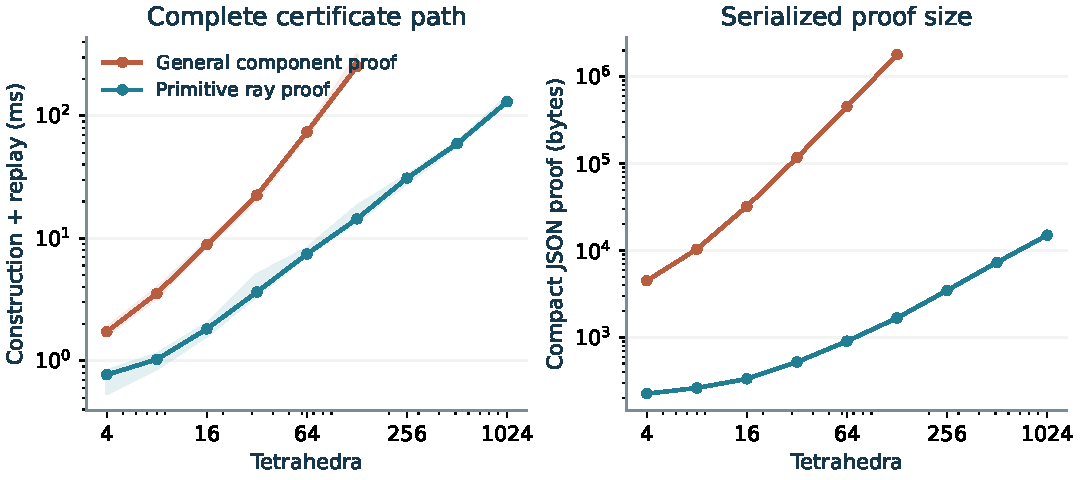
\includegraphics[width=\textwidth]{figures/primitive_ray_performance.pdf}
\caption{Full primitive-disc certificate paths on the Fibonacci family. Lines show medians; shaded time bands show the observed five-run range. The old path was measured only through 128 tetrahedra, so no later comparative speedup is asserted.}\label{fig:rays}
\end{figure}

\begin{center}\small
\begin{tabular}{@{}rrrrrr@{}}
\toprule
$t$ & Bits & Ray build (ms) & Replay (ms) & Rank operations & Proof bytes \\
\midrule
256 & 178 & 14.34 & 15.23 & 5,603 & 3,474 \\
512 & 355 & 29.42 & 28.79 & 11,235 & 7,314 \\
1024 & 711 & 66.58 & 65.69 & 22,499 & 14,994 \\
\bottomrule
\end{tabular}

\end{center}

At 1,024 tetrahedra the largest coordinate has 711 bits; the explicit normal-disc count is $F_{1029}-5$, far beyond a feasible expanded-sheet computation. The new producer and verifier take roughly 0.13 s combined. The recorded rank-operation counts at 256, 512 and 1,024 tetrahedra are 5,603, 11,235 and 22,499. These happen to follow $22t-29$ in this labeling; they are operation-counter observations, not a general fill-in theorem. The A/A general-ray control ratios range from 0.957 to 1.093.

\subsection{Propagation, caps and whole-suite correctness}

The exact standard-coordinate propagation search was run on the Fibonacci family through eight tetrahedra with branching prohibited. It returns the exact primitive meridian every time. It examines three original anchors before the first positive result, uses $4t-1$ LP calls and $t-1$ mandatory propagations, and makes no type guesses. The pivot counts are:
\[
\begin{array}{c|rrrrrrrr}
t&1&2&3&4&5&6&7&8\\\hline
\text{pivots}&7&59&163&354&702&1073&1688&2620.
\end{array}
\]
These measurements stop at the first witness. The all-anchor, arbitrary-$t$ zero-backdoor result comes from Section~\ref{sec:fibonacci}, not from extrapolating this table.

The literal five-tetrahedron trefoil fixture completes all 20 anchors negatively with 1,554 pivots, no branches and no mandatory updates. Its full negative certificate independently replays. A five-tetrahedron solid torus obtained by three $2$--$3$ moves needs one branch under the fixed policy. An empty permitted branch set is inconclusive; permitting tetrahedron 1 alone succeeds and exercises the fallback that branches inside $B$ even when the current conflict is elsewhere. These observations are deciding runs, not computed minima of the strong parameter.

The ten-tetrahedron figure-eight control exhausts its aggregate 10,000-pivot allowance after completing 21 of 40 anchors. It returns \status{INCONCLUSIVE} without a negative certificate. Its single exploratory run took about 79.48 s. This is an explicit limitation of the dense exact LP prototype, retained in the data rather than removed as an inconvenient benchmark. An interior-vertex positive-Euler control also fails the disc endpoint because its boundary class is zero, demonstrating the intended distinction between the two APIs.

The complete maintained-plus-new test discovery covers 1,287 unique successful test IDs. The initial sparse work layout omitted 14 pinned reference assets; this caused 13 import/data errors and no assertion failures. After restoring those unchanged assets, only the affected modules were rerun: 85 tests passed, with three previously successful tests repeated. The coverage record reconciles all 1,287 expected IDs with no missing or unexpected cases. Both the initial log and the recovery log are preserved. No production or test fixes were needed for that layout recovery.

Focused new tests include 240 exact random cones compared with exhaustive support-ray oracles; complete small-sector comparisons; interior and multiple boundary vertices; 20,000-bit coefficient transport; caps; cancellation; malformed and foreign proofs; omitted anchors and children; and verification with producer functions disabled. These checks support the implementation at the specified boundary. They do not replace the mathematical proofs or establish the missing global parameter theorem.

\section{Further research questions and proposed programme}\label{sec:research}

The next stage should aim to prove or refute sharply stated structural claims while improving the parts already justified. A favorable timing curve cannot substitute for a parameter theorem, and a parameter theorem should expose the algorithm that finds and preserves its useful structure. The following questions are ordered roughly by their effect on the recognition goal.

\subsection{Which propagation parameter is actually small?}

\textbf{Question 1: Can a useful logarithmic bound survive the unused-type obstruction?}
The mandatory-only strong backdoor requires every surviving mask to be compatible. A canonical positive witness avoiding a tetrahedron prevents any type there from becoming mandatory along the branch containing that witness. Thus harmless unused tetrahedra can force a large strong backdoor even when finding a positive surface is easy. Before proposing a universal bound, characterize this obstruction under a specified one-vertex reduction policy. Does that policy eliminate enough such freedom, or is the strong parameter fundamentally the wrong universal target?

A useful result would be either an explicit family of genuine knot-exterior triangulations with a proved linear lower bound after the permitted preprocessing, or a theorem bounding the obstruction for a rigorously specified class. Reducible torus-boundary manifolds and arbitrary abstract matching systems are valuable controls, but they cannot stand in for knot exteriors when asserting a lower bound relevant to unknot recognition.

\textbf{Question 2: Can the deciding-set parameter be bounded geometrically?}
Allowing a verified positive leaf before all unused masks are fixed removes the logical necessity behind the strong-mask obstruction. The resulting parameter depends on the exact LP witness and search policy. Find conditions under which a fixed polynomial LP policy has logarithmic deciding sets, or replace policy dependence by a geometric quantity with an explicit constructive reduction. A proof must control both negative branches and the time needed to discover a positive leaf; the mere existence of a short disc certificate does not bound search time.

\textbf{Question 3: Can useful sets be found in fixed-parameter time?}
Subset enumeration gives $(3t)^{O(b)}$, which is enough for a logarithmic quasi-polynomial target but loses a factor of $\log t$ in the exponent. Can a failed closure return a small obstruction set that every valid strong backdoor must meet? If so, branch on that obstruction and seek an $f(b)\poly(t)$ algorithm. One must prove that the obstruction covers \emph{all} valid sets, including sets whose choices alter the relaxed witness indirectly. The fixed-$B$ regression in this package shows why simply branching on the current LP witness's conflicts is insufficient for that purpose.

\subsection{Can the closure be made stronger without hiding hard work?}

\textbf{Question 4: What do forced-zero and dominance rules buy?}
Implement the optional whole-cone zero test and compare the resulting closure with mandatory-only propagation. Study whether it removes irrelevant masks and weakens the unused-type obstruction in genuine triangulations. A zero-coordinate certificate is a linear dual inequality, so its replay is straightforward. Its structural effect is not: coordinates can vanish on all admissible positive surfaces without vanishing on the relaxed cone, leaving a substantial gap.

For anchor objectives, go beyond componentwise dominance. A potential $\ell_a$ is removable from a vertex minimum if a retained $\ell_b\le\ell_a$ throughout $Q_S$; the inequality itself has a Farkas proof. More generally, test whether an anchor can ever be the unique minimum. Remove redundant anchors sequentially, retaining at least one representative of ties. Simultaneously removing every tied representative would destroy the minimum. The target is a certified reduction in anchor count, not an unproved claim that every lower envelope is small.

\textbf{Question 5: Which mixed normal constraints have a bounded proof width?}
The current rules use one forbidden coordinate at a time. Small sets of forbidden types may expose implications invisible to every singleton test. Define a bounded-width implication system, its certificate grammar and its exhaustive closure, then ask whether geometric classes admit small width. Cost must be charged for finding these implications: trying all $r$-sets costs $t^{O(r)}$. A new proof system is useful only if its stronger consequences repay that search and can be retained through topology transitions.

The abstract hardness result of Burton--He is a warning against treating arbitrary algebraic matching data as automatically easy \cite{BurtonHe}. It concerns an abstract normal-surface constraint problem and does not establish hardness of this genuine knot-exterior query. Any favorable theorem must identify the geometric restriction it exploits; any negative reduction must preserve that restriction.

\subsection{How should the exact solver and certificate backend improve?}

\textbf{Question 6: Can the current dense simplex bottleneck be removed?}
The figure-eight cap is a concrete target. The propagation code repeatedly rebuilds dense $7t$-coordinate LPs and starts cold. Test a revised sparse exact simplex, basis reuse across anchor objectives, and incremental deletion of forbidden columns. Investigate rational reconstruction from a numerical proposed basis with exact primal/dual acceptance checks. Report reconstruction failures and fallback costs as part of the result. A numerically plausible infeasibility claim must never become a negative certificate.

For an asymptotic implementation, provide a polynomial rational-LP backend with explicit encoded-size and support-recovery bounds. For a practical implementation, a rigorously checked hybrid may be substantially faster than a purely theoretical backend. These are separate evaluation criteria; both should be recorded.

\textbf{Question 7: Can the support kernel be maintained during propagation?}
After a mandatory deletion, some triangle equations become zero-labelled and their classes can merge. Rebuilding a contracted kernel should shrink the next LP, but it must preserve original row identities or a checkable row transformation for dual replay. A suitable data structure would maintain graph components, integer potentials, cycle constraints and the Euler covector under type deletions. The proof obligation is exact equivalence of the updated cone, including nonzero-labelled self-loops and inactive vertex-link factors. This is a natural connection to the project's earlier compiled-transfer work.

\textbf{Question 8: How small can negative proofs be made?}
The envelope reduced serialized proof bytes in the present audit, while increasing pivot count. Separate the optimization objectives of producer time, replay time and proof size. Intern repeated multipliers; retain a sparse set of original independent rows; or search for one dual dominating a family of anchor objectives. Determine when a compact covering family replaces all $P$ tuples with a coverage proof of polynomial size. The sharp anchored-standard determinant bound suggests small numerators exist; it does not ensure that the present solver discovers the sparsest or shortest such certificate.

An important test is whether a compressed negative proof can be verified without reconstructing the very exponential enumeration it replaces. A list of anchor hashes is not a coverage proof; a compressed proof grammar must have an independently checked meaning.

\subsection{How does the structure behave under topology changes?}

\textbf{Question 9: Is there a transition-stable potential controlling branch work?}
Measure and then analyse the chosen parameter before and after one-vertex conversion, Pachner moves, boundary simplification and crushing. A useful theorem might bound an amortized sum of branch exponents along the full recognition trajectory rather than bounding every stage separately. Conversely, construct examples where a locally attractive reduction sharply increases the parameter. An amortized result must count all visited states, including unsuccessful alternative reductions, rather than only the ultimately successful path.

The infinite-family Fibonacci proof offers a model: matching identities expose local forced choices that survive all anchors. Seek analogous symbolic identities in more general layered blocks, cables and gluing constructions, keeping peripheral information explicit. Prove how forcing relations compose across an interface before claiming that a small interface bounds global choices.

\textbf{Question 10: Can hierarchy and parallelity data produce certified implications?}
Lackenby's hierarchy work provides a distinct geometric route involving normal surfaces and controlled decompositions \cite{Lackenby2026}. Investigate whether parallelity regions or boundary-pattern simplifications can be translated into LP implications, compressed interface states or a bound on deciding sets. The relationship is presently a research question; no result in that paper identifies its hierarchy complexity with $k$, $d$ or $\beta_{\mathrm{LP}}$ here.

For interface methods, a bounded number of ports is not enough by itself: normal multiplicities are unbounded integers. Any finite-state or bounded-width claim must explain exactly which arithmetic information is retained, how its bit length is controlled, and why gluing preserves feasibility and essentiality. The earlier topology-spectrum and sparse-incidence continuations are relevant foundations for this question.

\subsection{How should the evidence and trust boundary expand?}

\textbf{Question 11: Where does the sector LP actually beat enumeration?}
The frozen audit has only 30 sectors of nullity five and none of higher nullity. Extend it with topology-validated, source-frozen families that increase nullity, active vertex count and coefficient bit length independently. Include incompressible knot exteriors, easy positive controls, deliberately awkward triangulations, and repeated refinements of the same manifold. Select benchmark cases by structure before timing, retain all outcomes and caps, and report both distinct surfaces and repeated sector outputs. This will identify a defensible hybrid dispatch rule and show whether a practical crossover exists on relevant inputs.

\textbf{Question 12: Can primitive-ray verification become uniformly complete and nearly linear?}
The fixed-prime rank strategy is sound but not complete. Provide a deterministic prime schedule with a proved stopping bound from the matching minor height, or a fraction-free fallback. Study fill-in on topology-derived support matrices and reuse rank witnesses along source-certified triangulation transformations. A proposed nearly linear bound must include manifold validation, coordinate arithmetic, boundary homology and source binding, not merely a fast elimination kernel.

Extend the short proof only where its hypotheses justify it. Primitive nonextreme vectors need not be connected, and Euler/parity alone fail on the M\"obius-plus-link example. A broader endpoint could combine small-rank decomposition with the existing compressed component certificates, but must preserve one-sided and multiplicity behavior.

\textbf{Question 13: What is the smallest complete independently checked recognition pipeline?}
Integrate diagram provenance, candidate search, primitive-ray or general geometry replay, and topology-preserving reduction certificates. State every terminal rule and every base case, and run the complete pipeline on both unknots and nontrivial knots. For a negative decision, retain a checked exhaustion or hierarchy proof; for a positive decision, retain an authenticated essential disc. This integration is a prerequisite for comparing end-to-end recognition latency rather than isolated surface queries.

Formalization can then begin with the small arithmetic core: nonnegative-kernel dual soundness, modular rank lower bounds, gcd/primitivity, anchor coverage and propagation-tree semantics. The difficult topology boundary should be named explicitly rather than hidden behind a Boolean validator. A useful first formal milestone is a theorem that every accepted negative proof excludes the specified canonical surface class, with a separate theorem connecting that class to a complete knot-exterior algorithm.

\subsection{Suggested order of work}

The immediate engineering sequence is: integrate the primitive-ray fast path with its fallback; build sparse/reused LP state against the figure-eight cap; and add the closure refinements with independent dual replay. In parallel, the mathematical priority is to test the strong-backdoor obstruction and develop a parameter that captures early positive termination without hiding policy-dependent search. Only after that should a universal logarithmic conjecture be promoted to the main target.

The next research report should have three concrete deliverables: a substantially larger frozen high-nullity corpus with paired query timings; either a proved useful family bound or a genuine knot-exterior lower-bound construction for the selected parameter; and a source-bound search-and-reduction integration prototype. Those deliverables would turn the present conditional complexity statement into a sharper, falsifiable programme.

\appendix
\section{Reproducing and reviewing the delivery}\label{sec:reproduce}

\subsection{Package contents and source provenance}

The archive contains this PDF, the complete modular \LaTeX{} source, generated tables and publication figures, a frozen \code{fast/} runtime with the new modules and tests, minimal unchanged report/synthesis test references, exact oracle and certificate JSON, raw measurement observations, test logs, reproduction scripts, and an additive \code{integration.patch}. A top-level README states the query contracts and integration scope.

The maintained source is pinned to \baseline. The earlier sector modules and arbitrary-size Fibonacci constructor are identified as unchanged incoming dependencies. The new files are listed separately in \code{PROVENANCE.json}. Contextual source hashes in provenance and experiment records bind results to their code and inputs; there is no checksum-only manifest. The snapshot's MIT No Attribution license is retained, and external reference files keep their original notices.

The archive's \code{fast/} directory excludes unrelated historical benchmark result dumps and Python caches. Small original reference files needed by the maintained tests are included at their expected sibling paths under \code{reports/} and \code{synthesis/}. These are executable test dependencies, not imported full reports. The new Fibonacci fixture is also available at \code{fast/fibonacci_fixture.py}, so the added test can be integrated with the maintained test command without relying on a separate report's scripts directory.

\subsection{Standard-library certificate replay}

From the extracted archive root, run:
\begin{lstlisting}[language=bash]
python3 scripts/replay_certificates.py
\end{lstlisting}
The verifier-only driver inventories every saved non-null certificate field and rejects unhandled proof objects. It replays 14,773 certificates: 7,314 ordinary sector proofs, 7,314 envelope-strategy proofs, 117 standalone ray proofs, 14 propagation case proofs, 12 nested disc proofs and two redundant negative-tree controls. It imports no LP producer, enumerator or Regina module. Incomplete records and Boolean-only historical observations are reported separately and do not inflate that count.

The default output is \code{results/reproduced/certificate_replay.json}. Frozen inputs are protected against accidental overwrite. The new replay record can be compared with the delivered record by counts and accepted claims; diagnostic elapsed time is not expected to reproduce byte-for-byte.

\subsection{Tests and full audits}

The focused tests can be run without external numerical packages:
\begin{lstlisting}[language=bash]
PYTHONPATH=fast:scripts python3 -m unittest discover \
  -s fast/tests -p 'test_normal_euler.py' -v
PYTHONPATH=fast:scripts python3 -m unittest discover \
  -s fast/tests -p 'test_normal_ray.py' -v
PYTHONPATH=fast:scripts python3 -m unittest discover \
  -s fast/tests -p 'test_normal_propagation.py' -v
\end{lstlisting}
The full maintained-plus-new discovery uses \code{-s fast/tests -v}. Some maintained or optional checks use Regina; the recorded complete run enabled the 7.4.1 wheel. Its exact environment, restored reference assets and unique-ID reconciliation appear in the delivered test records.

To repeat the frozen-oracle audits rather than only replay proofs:
\begin{lstlisting}[language=bash]
python3 scripts/audit_normal_ray.py \
  --output results/reproduced/ray_audit.json
python3 scripts/audit_sector_euler.py \
  --output results/reproduced/sector_euler_audit.json
\end{lstlisting}
These commands use the supplied complete ray lists and do not regenerate Regina's triangulations. The sector audit reruns the old enumerator and both new LP strategies, so it does more work than certificate replay. Its output should reproduce decisions, coverage and exact counters under the same source; one-shot timings are incidental.

The saved propagation audit includes literal finite triangulations, every selected option and result, and the bounded figure-eight case. The focused propagation tests reconstruct its principal controls. The package also supplies a reproduction script for its saved case requests, preserving the exact fixture labels and options. Do not compare a newly simplified or isomorphism-signature relabelled trefoil against the literal audit's pivot count without recording that input change.

\subsection{Benchmarks and document build}

For controlled measurements, stop other local CPU-heavy work first and run:
\begin{lstlisting}[language=bash]
python3 scripts/benchmark_dual_continuation.py --repeats 5 \
  --output results/reproduced/controlled_benchmarks.json
\end{lstlisting}
This uses predeclared structural selection and randomized A/A/B ordering. The golden tables use the delivered \code{results/controlled_benchmarks.json}; copying a newly produced measurement into that role is an intentional new experiment, not a silent reproduction step. The figure/table script requires Matplotlib and reads those frozen golden measurements:
\begin{lstlisting}[language=bash]
python3 scripts/make_tables_and_figures.py
latexmk -pdf -interaction=nonstopmode -halt-on-error \
  -cd article/unknot_dual_certificates.tex
\end{lstlisting}
The figures are included in PDF, SVG and PNG formats. The article compiles with ordinary pdf\LaTeX{}, Latin Modern and standard mathematical packages; no proprietary fonts, shell escape or external bibliography service are required. The delivered PDF was rendered and inspected after compilation.

\subsection{Patch review}

The patch is an additive proposal relative to the pinned repository. It imports the two earlier sector modules and Fibonacci fixture, then adds the seven new producer/verifier modules and three focused test files. It does not change the recognizer's default dispatch or claim to integrate crushing. A maintainer can inspect or check the patch independently of placing this report. The original delivery is intended for the repository's numbered report collection; deployment and default-policy decisions belong to the subsequent integration step.

\begin{thebibliography}{99}
\raggedright
\addcontentsline{toc}{section}{References}

\bibitem{ProveIt}
V.~Reshetnikov and ProveIt contributors,
\emph{ProveIt: Unknot recognition research and incoming reports}.
Repository snapshot \baseline, inspected 9 October 2026.
\href{https://github.com/VladimirReshetnikov/ProveIt/tree/3a90fb34146c915328ab8eac6250cc2514f74ed0/Topology/UnknotRecognition}{Pinned unknot-recognition source tree}.
Incoming directory:
\href{https://github.com/VladimirReshetnikov/ProveIt/tree/3a90fb34146c915328ab8eac6250cc2514f74ed0/docs/incoming}{Pinned incoming directory}.

\bibitem{priorKernel}
ProveIt research continuation,
\emph{Quadrilateral Support Kernels and Certified Normal-Disc Discovery},
9 October 2026. Incoming archive
\code{unknot_quadrilateral_support_kernel_20261009.zip} at the pinned snapshot.
\href{https://github.com/VladimirReshetnikov/ProveIt/blob/3a90fb34146c915328ab8eac6250cc2514f74ed0/docs/incoming/unknot_quadrilateral_support_kernel_20261009.zip}{Pinned source archive}.
The contraction, mixed-minor estimate, canonical ray lifting and earlier layered support obstruction are dependencies of this continuation.

\bibitem{HLP}
J.~Hass, J.~C. Lagarias and N.~Pippenger,
\emph{The computational complexity of knot and link problems},
Journal of the ACM \textbf{46} (1999), no.~2, 185--211.
\url{https://arxiv.org/abs/math/9807016}.

\bibitem{Tollefson}
J.~L. Tollefson,
\emph{Normal surface Q-theory},
Pacific Journal of Mathematics \textbf{183} (1998), no.~2, 359--374.
\url{https://msp.org/pjm/1998/183-2/pjm-v183-n2-p07-s.pdf}.

\bibitem{BurtonQ}
B.~A. Burton,
\emph{Converting between quadrilateral and standard solution sets in normal surface theory},
Algebraic \& Geometric Topology \textbf{9} (2009), 2121--2174.
\url{https://arxiv.org/abs/0901.2629}.

\bibitem{Suh}
C.~Suh,
\emph{The unknotting problem and normal surface Q-theory},
arXiv:1009.1500, first submitted 8 September 2010.
\url{https://arxiv.org/abs/1009.1500}.

\bibitem{BO}
B.~A. Burton and M.~\"Ozlen,
\emph{A fast branching algorithm for unknot recognition with experimental polynomial-time behaviour},
arXiv:1211.1079v3, 9 October 2014.
\url{https://arxiv.org/pdf/1211.1079}.
Numbering in this report refers to version~3: Algorithm~9, Lemmas~5--10 and Theorems~11--12.

\bibitem{AHT}
I.~Agol, J.~Hass and W.~P. Thurston,
\emph{The computational complexity of knot genus and spanning area},
arXiv:math/0205057v2, 10 July 2004.
\url{https://arxiv.org/abs/math/0205057}.

\bibitem{BurtonHe}
B.~A. Burton and A.~He,
\emph{On the hardness of finding normal surfaces},
Journal of Applied and Computational Topology \textbf{5} (2021), 583--619.
\url{https://arxiv.org/abs/1912.09051v3}.

\bibitem{Khachiyan}
L.~G. Khachiyan,
\emph{A polynomial algorithm in linear programming},
Doklady Akademii Nauk SSSR \textbf{244} (1979), no.~5, 1093--1096.
\url{https://www.mathnet.ru/eng/dan42319}.

\bibitem{Bland}
R.~G. Bland,
\emph{New finite pivoting rules for the simplex method},
Mathematics of Operations Research \textbf{2} (1977), no.~2, 103--107.
\url{https://doi.org/10.1287/moor.2.2.103}.

\bibitem{LackenbyTalk}
M.~Lackenby,
\emph{Unknot recognition in quasi-polynomial time},
Oxford seminar slides, March 2021, 34-page handout.
\url{https://people.maths.ox.ac.uk/lackenby/quasipolynomial-talk-oxford-compressed.pdf}.
The displayed announced bound is $2^{O((\log n)^3)}$.

\bibitem{Lackenby2026}
M.~Lackenby,
\emph{Incompressible surfaces, hierarchies and unknot recognition},
arXiv:2607.23350v1, 25 July 2026.
\url{https://arxiv.org/abs/2607.23350}.
Section~9 distinguishes iteration bounds from an implementation running-time estimate; this report does not import a quasi-polynomial runtime theorem from that paper.

\end{thebibliography}

\end{document}
